\chapter{自适应的极大二分团枚举数据结构}
\label{ch:adapt_mbe}

针对极大二分团枚举问题中静态数据结构效率低下的问题,本章整理了相关工作中不同的图存储数据结构,详细描述不同数据结构的优劣以及适用场景,并指出静态数据结构所导致的局限性,作为本章的研究出发点。
具体而言,现有算法通常使用静态图结构完成枚举,但忽略了枚举过程中子图动态变化的特性,导致在原图中进行大量无效内存访问;同时,现有算法采用邻接表存储二分图,导致高昂的集合运算开销。在这些因素的限制下,现有算法仅能处理包含不超过1亿极大二分团的小数据集。为了解决这些问题,本章提出以下优化方法:首先,本章提出了基于局部计算子图的优化方法,通过动态缓存枚举过程中的计算子图,优化算法的枚举过程,从而减少无效的顶点访问、集合运算和枚举节点。然后,本章提出了基于位图的动态子图方法,利用位图加速了小计算子图中的集合运算。最后,本章结合上述两个技术点,形成自适应的极大二分团枚举算法AdaMBE。实验证明,AdaMBE算法相比于现有工作的运行时间缩短1.6-49.7倍,并成功应用于超过190亿极大二分团的TVTropes数据集。

% 具体而言,现有算法通常采用邻接表结构存储二分图,在进行大量集合交集运算时会带来较高的计算开销;同时,过多地访问顶点的全部邻居也存在冗余计算问题。这些因素限制了算法只能应用于包含不超过1亿极大二分团的小数据集。为了解决这些问题,本章提出以下优化方法:首先,针对邻接表上集合运算的高开销问题,本章提出基于位图的动态子图方法。该方法在计算过程中动态生成子位图,通过在子位图中进行集合运算,提升集合运算的效率。然后,针对访问顶点完整邻居导致的冗余计算问题,本章提出基于局部计算子图的优化方法。该方法通过动态保存顶点的部分活跃邻居,避免大量对结果无影响的不活跃邻居的访问,从而减少冗余计算。此类冗余计算包括对含有非极大二分团的节点的计算、重复的集合运算以及无效顶点的访问。最后,本章结合基于位图的动态子图方法和基于局部计算子图的优化方法,形成自适应的极大二分团枚举算法AdaMBE。实验证明,AdaMBE算法相比于现有工作的运行时间缩短1.6-49.7倍,并成功应用于超过190亿极大二分团的TVTropes数据集。



\section{二分图的存储结构}
\label{subsec:ada_representation}

二分图的存储结构对极大二分团枚举算法中集合运算的效率具有直接影响,在极大二分团枚举过程中扮演着关键角色。图~\ref{fig:ada_graph_format}展示了图~\ref{fig:ada_eg_tree}中二分图$G_2$的三种二分图存储结构,包括邻接表、位图和哈希表。每种数据结构在时间和空间开销上都有其独特的优势和局限性,因此在实际应用中需要权衡各种因素,选择最适合的存储结构解决问题。

\begin{figure} [H]
  \centering
  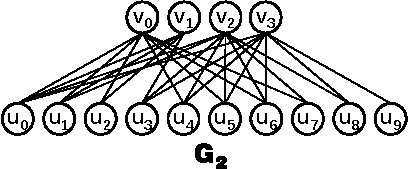
\includegraphics[width=0.5\linewidth]{adambe/eg_graph.pdf}
  \caption{二分图$G_2$}
  \label{fig:ada_eg_tree}
\end{figure}


\begin{figure} [H]
	\centering
  \vspace{0.1in}
	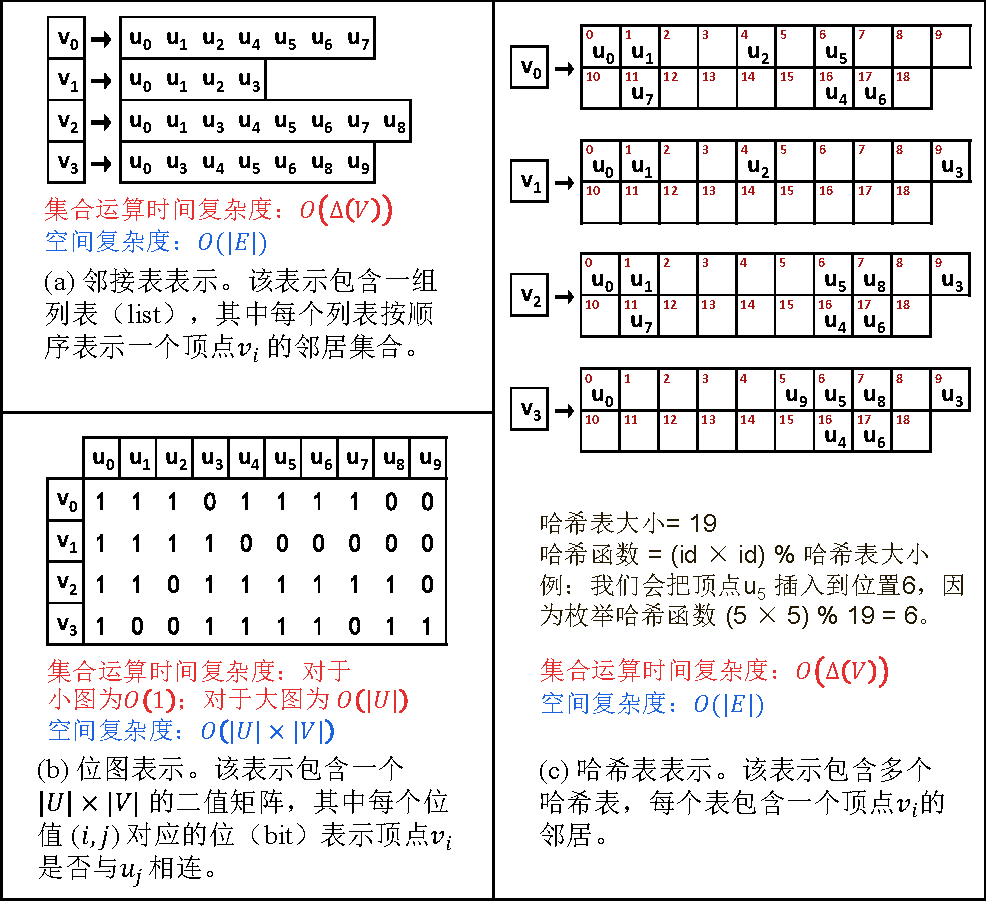
\includegraphics[width=0.9\linewidth]{adambe/eg_representation_full}
  \vspace{0.2in}
	\caption{二分图$G_2(U,V,E)$的三种存储结构}

	\label{fig:ada_graph_format}
\end{figure}

\textbf{邻接表:} 邻接表是一种常见的图存储结构,具有\emph{低存储使用}的优点,特别适用于稀疏图。在邻接表中,每个顶点都与一个包含其相邻顶点的链表相关联。这种存储结构节约内存,因为它只存储实际存在的边,而不需要额外的空间来存储缺失的边,因此它的空间开销仅为$O(|E|)$。此外,邻接表使得遍历图变得更加高效,因为我们可以通过遍历每个顶点的邻居链表来访问相邻顶点。邻接表在许多图算法中表现良好,特别是针对稀疏图的算法。然而,对于集合交集运算,邻接表可能会受到顶点度数较大的影响,因为每次交集操作都需要按顺序访问一个顶点的邻居,时间复杂度为$O(\Delta(V))$。在处理稠密图时,邻接表可能不如其他存储结构效率高,因为缺失的边在这类图中的占比较小,导致邻接表的低存储使用的优势无法凸显。邻接表存储结构广泛应用于最新的极大二分团枚举算法中,例如PMBE~\cite{PMBE20}和ooMBEA~\cite{ooMBE22}。

\textbf{位图:} 位图是另一种常见的图存储结构,在小图中具有\emph{计算高效}的特点,可以通过位运算实现集合交集运算,通常用于小图或密集图的存储。如图~\ref{fig:ada_graph_format}所示,在位图中,每个元素即一个位(Bit),代表两个顶点的连接关系。与邻接表不同,位图在执行集合交集操作时不受顶点度数限制,因为它直接对应于所有可能的边。这使得位图在处理高度连通图时表现出色。在二分图中,通过两个$|U|$位的位图之间进行按位与操作(\&),可以计算出两个顶点的共同邻居,这个集合交集运算的时间复杂度为$O(|U|)$。对于小图,通过几次按位与操作,它可以在$O(1)$ 内高效地执行集合交集。然而,位图可能需要大量内存,特别是对于大规模稀疏图,因为需要为所有缺失的边分配位。这可能会导致内存消耗过大,不适用于资源有限的情况。因此,位图存储结构仅应用于早期的基于小图的极大二分团枚举算法中,包括 LCM-MBC~\cite{lcmmbc07} 和 iMBEA~\cite{iMBEA14}。

\textbf{哈希表:} 哈希表是一种基于散列函数的数据结构,适用于\emph{快速查找和插入元素}的场景。在哈希表存储法下,二分图中每个顶点的邻居存放在一张哈希表中,每张哈希表通过哈希函数,能够在$O(1)$的时间内快速地查找某顶点是否在这张哈希表中。因此,在实现集合交集操作$A \cap B$时,假设集合$A$顶点数多于集合$B$的顶点数,我们可以通过将集合$B$中的每个元素分别在集合$A$对应的哈希表中进行查找的方式实现,因此集合交集运算的复杂度为$O(|B|)$。由此可知,哈希表在两个输入集合差异显著时,计算效果尤为明显。同时,部分完美哈希函数~\cite{cuckoohash04,murmurhash}能够实现空间复杂度与输入集合长度相同,因此得到与邻接表类似的空间复杂度。基于哈希表的存储结构,Jovan等人优化了极大团枚举算法的时间复杂度~\cite{MCE20}。然而,相比于邻接表,哈希表存储结构可能涉及大量的随机内存访问和更高的内存使用,效率不够理想。哈希表存储结构仅在 ParMBE~\cite{parMBE19} 中使用。


% 在图的表示中,哈希表通常用于某些特定的图算法。哈希表表示法通过高效的查找操作加速集合交集操作,尤其是在输入集大小差异显著时。虽然哈希表与邻接表具有类似的时间和空间复杂度,但可能涉及大量的随机内存访问和更高的内存使用。这可能导致性能相对较低,与邻接表相比效率不够理想。然而,在某些需要快速查找和动态更新的图算法中,哈希表表示法可能是更好的选择。哈希表表示法还可以处理图中的边属性信息,使得它在某些情况下更加灵活和实用。哈希表表示法仅在 ParMBE~\cite{parMBE19} 中使用。
\section{研究出发点}

尽管现有研究已经提出了许多优化方法来提高枚举效率,但现有的极大二分团枚举算法通常在单一的静态图结构下完成枚举,忽略了枚举过程中计算子图动态变化的特性,导致算法的性能受到静态数据结构的限制。本节将现有算法的数据结构限制归纳为两个方面:在原图中的大量无效内存访问和在邻接表上高昂的集合运算开销,并结合例子进行说明。为了方便表述,本章中默认以算法~\ref{alg:se_mbe} 在二分图$G_2$上的集合枚举树为例,如图~\ref{fig:ada_tree}所示。


% 尽管已经有许多算法上的方法优化了极大二分团枚举问题的搜索空间,但是它们忽略了由数据结构限制带来的固有的计算低效性问题。这导致现有的算法只能应用于包含不超过1亿极大二分团的小数据集。因此,在本节中,我们将概括现有方法的数据结构限制,主要包括邻接表上进行集合运算的高计算开销以及算法中默认重复访问顶点的完整邻居带来的冗余计算。同时,我们将通过例子进行说明。为了方便表述,本章中默认以算法~\ref{alg:se_mbe} 在二分图$G_2$上的集合枚举树为例,如图~\ref{fig:ada_tree}所示。

\begin{figure} [t]
	\centering
  \vspace{0.1in}
	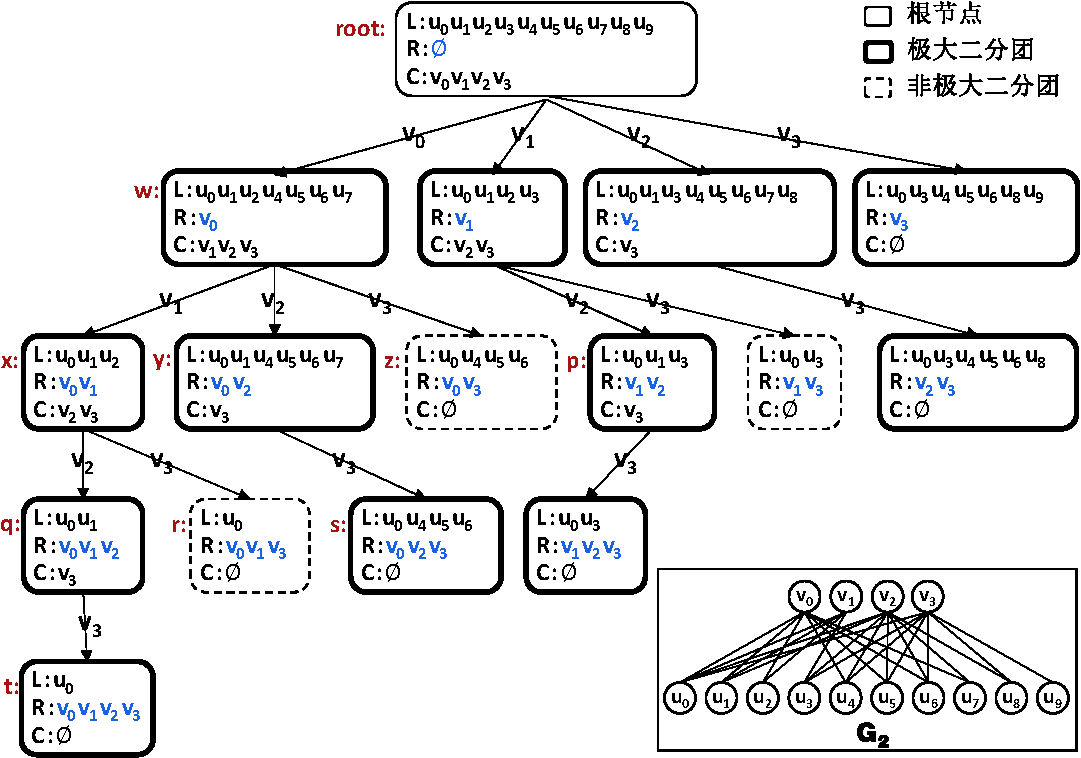
\includegraphics[width=0.95\linewidth]{adambe/eg_tree}
  \vspace{0.2in}
	\caption{算法~\ref{alg:se_mbe}在二分图$G_2$上的集合枚举树}

	\label{fig:ada_tree}
\end{figure}

\subsection{原图中大量的无效内存访问}
\label{subsec:ada_limitation_vertex}

目前,现有的极大二分团算法通常以静态方式存储原始二分图,并在计算过程中直接访问原图中的顶点。然而,我们观察到由活跃顶点产生的计算子图在枚举过程中会动态变化。\emph{访问原图中不在当前计算子图的顶点对计算结果并无影响,因此是无效的。}这导致现有方法中存在大量的无效内存访问,从而造成性能瓶颈。本节首先定义了计算子图,然后给出了三个关于计算子图特征的逐步深入的观察,最终结合实验数据指出了现有方法的不足之处。

\begin{definition}

	\textbf{(计算子图)} 对于当前节点$(L,R,C)$,极大二分团枚举算法中的计算子图指的是由$L$和$C$中顶点组成的子图,该子图包含原始二分图中$L$和$C$中的所有边。在后续内容中,我们使用 CG 表示计算子图。

\end{definition}

结合~\ref{subsec:baseline}节提到的算法~\ref{alg:se_mbe} 以及该算法在真实数据集上的执行结果,关于计算子图的特征,我们得到以下三个逐步深入的观察:


\begin{itemize}
\item \textbf{O1:计算子图是大小动态变化的。} 根据计算子图的定义,每个节点的$|L|$和$|C|$大小不同,因此计算子图的大小也会随着节点$|L|$和$|C|$的大小动态变化。为了进一步说明这一点,我们进行了一系列实验,并在图~\ref{fig:distribution} 中展示了在BookCrossing和Github数据集上计算图大小的频率分布情况。图中的每个单元格表示特定$|L|$和$|C|$组合在计算子图中出现的频率,并已用总出现次数对频率进行了归一化处理。值得注意的是,相对于原图,大多数计算子图相对较小,其中90\%的计算子图中的$|L|$和$|C|$均小于32。

% 例如,在图~\ref{fig:distribution} 中,我们发现90\%的计算子图包含的$|L|$和$|C|$都小于32。

\begin{figure} [H] 
	\centering
    \subfloat[BookCrossing.]{
		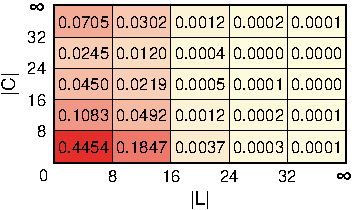
\includegraphics[width=0.46\linewidth]{adambe/distribution_bx}
		\label{fig:distribution_bx}
	}
  \subfloat[Github.]{
		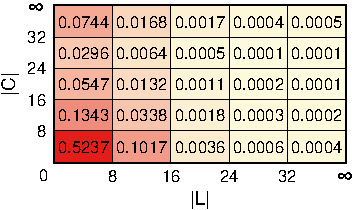
\includegraphics[width=0.46\linewidth]{adambe/distribution_gh}
		\label{fig:distribution_gh}
	}

	\caption{基于$|L|$和$|C|$大小的计算子图频率分布图}
	% 基于$|L|$和$|C|$的CG大小分布。每个单元格表示特定$|L|$和$|C|$组合的出现频率,用总出现次数进行归一化。
	\label{fig:distribution}

\end{figure}



\item \textbf{O2:当前枚举节点的计算子图可直接用于节点生成。} 具体而言,在算法~\ref{alg:se_mbe}中,当前节点$(L, R, C)$通过遍历$v'$生成节点$(L', R', C')$。我们知道$L'$是$L$的子集(第4行)。根据我们的观察,在节点生成过程中,我们可以将对原图上顶点邻居的访问全部替换为对当前计算子图内顶点局部邻居的访问。具体而言,我们将$L \cap N(v')$(第4行)推导为$L \cap N(v') = L \cap (L \cap N(v'))$,并将$L' \cap N(v_c)$(第6、8行)推导为$L' \cap N(v_c) = (L' \cap L) \cap N(v_c) = L' \cap (L \cap N(v_c))$,其中$L \cap N(v')$和$L \cap N(v_c)$表示当前计算子图中顶点$v'$和$v_c$的局部邻居。这样的替换方式可以减少对原图的访问次数,进而提高算法的效率。

\item \textbf{O3:现有算法需要访问其当前计算子图外的顶点。} 尽管计算子图可以直接用于节点生成,但现有算法默认访问原图。然而,这种做法导致大量对当前计算子图外的无效的顶点访问,严重影响了算法的计算性能。如图~\ref{fig:ada_motivation_redundancy}所示,在绝大多数数据集上,这些无效的顶点访问占据了超过90\%的内存访问量,尤其在耗时较长的BookCrossing数据集上,这一比例高达99.9\%。

\begin{figure} [H]
	\centering
	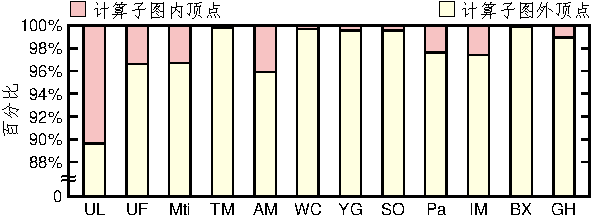
\includegraphics[width=0.8\linewidth]{adambe/redundancy_vertex}
	\caption{真实数据集中计算图内外顶点访问百分比  }
	\label{fig:ada_motivation_redundancy}
	% \vspace{-0.2in}
\end{figure}

\end{itemize}

总而言之,现有的方法在计算过程中默认对原图进行操作,导致了大量的计算子图外的无效顶点访问。如果我们能够充分利用计算子图内的内存访问,就能在减少无效顶点访问的同时,进一步减少重复集合运算和节点剪枝的操作,从而带来更大的优势。我们将在~\ref{subsec:ada_design_2}节进行详细说明。


\subsection{邻接表上高昂的集合运算开销}

% \begin{table} [t]
	\centering    
	\setlength{\abovecaptionskip}{0.2cm}  
   \setlength{\belowcaptionskip}{0cm}
	\caption{MBE问题中集合运算时间以及冗余邻居访问占比}      
	\label{tbl:ada_motivation}
  \setlength{\tabcolsep}{2pt}
	\begin{center}
				\normalsize{
          \begin{tabularx}{0.95\linewidth}{|>{\centering\arraybackslash}X|*{12}{>{\centering\arraybackslash}p{0.75cm}|}}
            \hline
            \textbf{数据集} &\textbf{UL} & \textbf{UF} & \textbf{Mti} & \textbf{TM} & \textbf{AM} & \textbf{WC} & \textbf{YG} & \textbf{SO} & \textbf{Pa} & \textbf{IM} & \textbf{BX} & \textbf{GH}\\
            \hline
            \textbf{集合运算时间占比 \%} & 55.8&	52.6&	65.9&	31.5&	55.8&	38.1 & 70.0&	73.4&	35.7&	58.2&	76.4&	85.4\\
            \hline
            \textbf{冗余邻居访问占比 \%} & 89.6&	96.6&	96.7&	99.8&	95.9&	99.7 & 99.5&	99.5&	97.6&	97.4&	99.9&	98.9\\
            \hline
          \end{tabularx}
				}
	\end{center}

\end{table}


近年来,极大二分团枚举算法通常以邻接表作为存储二分图的首选方式。这主要是因为在处理大规模稀疏图的情况下,相比于其他图存储结构,邻接表结构具有最小的存储开销~\cite{PMBE20,ooMBE22}。然而,\emph{基于邻接表进行集合操作需要对两个集合对应的邻接表进行顺序串} \emph{行比较,带来较大的计算开销。}
% 通过对基准算法MBEA~\cite{iMBEA14}在真实数据集中的实验统计,我们发现\emph{邻接表上的集合交集运算时间总是占据大部分的总运行时间}。表~\ref{tbl:ada_motivation}中的数据显示,在大多数数据集中,基于邻接表的集合交集运算耗时占据超过50\%的总运行时间,尤其在耗时最长的Github数据集上高达85.4\%。因此,优化基于邻接表的集合交集运算对于极大二分团枚举算法具有巨大的优化潜力。
具体而言,在图~\ref{fig:adambe_intersection} 中我们比较了邻接表与位图的集合运算实例。由于邻接表采用顺序连续存储的方式,进行集合操作通常需要串行访问和比较,导致操作时间与集合大小成正比,效率较低。相比之下,位图始终以等长方式存储顶点的所有邻居,因此每次集合操作可以通过固定长度的位运算(如与操作)实现。对于小规模的稠密图,位图能够在常数时间内高效执行集合操作;然而,对于大规模稀疏图,由于其较高的内存需求,使用位图变得不切实际。因此,我们需要一种能平衡内存消耗和集合操作效率的自适应数据结构。


% 根据表~\ref{tbl:ada_motivation} 的数据,邻接表上的集合交集可能占据超过 50\% 的运行时间,这也是极大二分团枚举过程中主要的计算时间消耗部分,具有很高的优化潜力。

% 然而,表~\ref{tbl:ada_motivation} 表明,邻接表上的集合交集可能占据超过 50\% 的运行时间,主要是由于对顶点邻居的顺序访问所致。我们在图~\ref{fig:adambe_intersection} 中通过比较邻接表与位图的集合运算实例,对邻接表上的集合运算低效性进行进一步阐述。虽然位图表示能够通过位运算与操作(\&)实现高效的集合交集运算,但对于大规模二分图来说,由于其高内存需求,变得不切实际。因此,需要一种平衡内存使用和集合运算时间的自适应的数据结构。

\begin{figure} [t]
	\centering
	% \vspace{0.1in}
	\subfloat[邻接表]{
		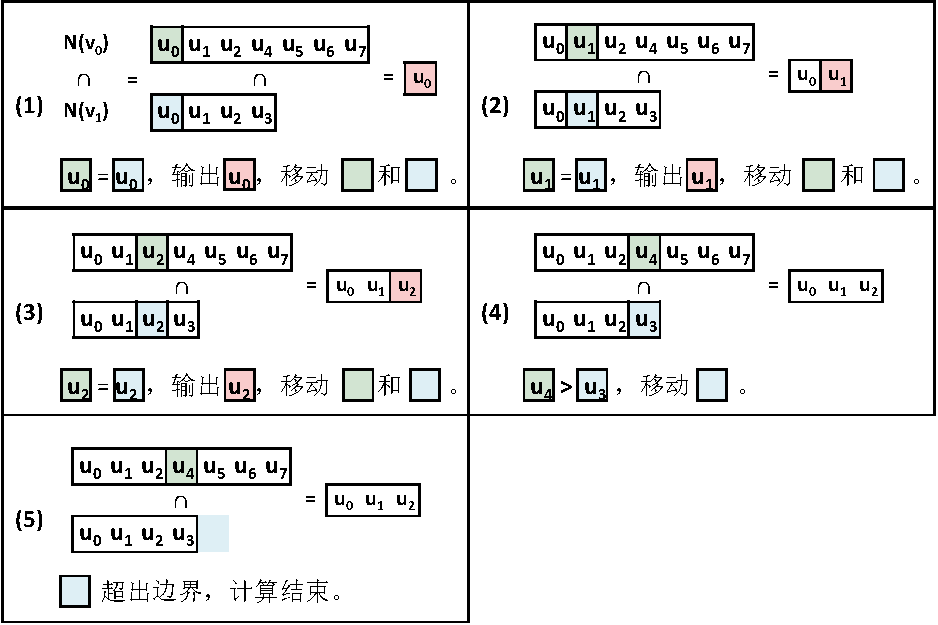
\includegraphics[width=0.7\linewidth]{adambe/eg_intersection_adjlist}
		\label{fig:adambe_intersection_adjlist}
	}
  \\
	\subfloat[位图]{
		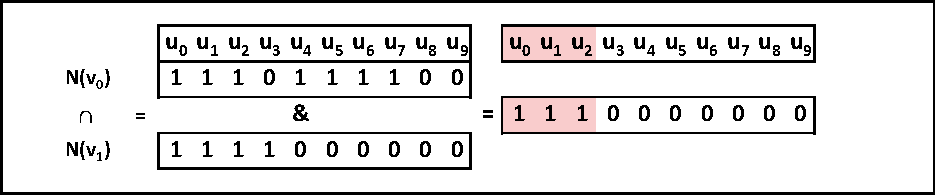
\includegraphics[width=0.7\linewidth]{adambe/eg_intersection_bitset}
		\label{fig:adambe_intersection_bitset}
	}
	% \vspace{0.1in}
	\caption{邻接表与位图的集合交集运算比较实例$N(v_0)\cap N(v_1)$}
	
	\label{fig:adambe_intersection}
\end{figure}


\begin{example}
	
	图~\ref{fig:adambe_intersection}展示了二分图$G_2$上$v_0$和$v_1$的共同邻居在邻接表和位图中的计算过程。图~\ref{fig:adambe_intersection_adjlist}则展示了一种基于邻接表的集合交集运算计算过程,采用双指针法。具体而言,首先,我们初始化两个指针,分别指向两个已排序集合的起始位置,并在集合中用绿色和蓝色标记指针位置。随后,我们不断地比较两个指针指向的元素。如果相等,则将该元素添加到交集中,并同时将两个指针向后移动一位(步骤\Num1、\Num2、\Num3);如果不相等,则将指向较小元素的指针向后移动一位(步骤\Num4)。最后,我们重复以上过程,直到其中一个集合的指针到达末尾为止(步骤\Num5)。除双指针法外,基于邻接表的集合运算方法还包括融合路径法~\cite{GpuMergePathIntersect14,MergePath18}、二分法~\cite{BinaryIntersect18,triangle18}等。然而,由于邻接表顺序连续存储的特性,集合运算至少需要对两个输入集合中的一个进行串行顺序访问。这意味着集合运算所需的时间与集合的大小直接相关,导致了较低的运算效率。
	
	图~\ref{fig:adambe_intersection_bitset}展示了一种基于位图的集合交集运算计算过程,采用位运算。具体来说,在二分图$G_2(U,V,E)$中,集合$V$中每个顶点$v$的邻居存储在一个长度为$|U|$的位图中,其中每一位代表$v$的邻居中是否存在对应元素。在位图存储下,我们通过对两个位图进行按位与(\&)操作,即可得到运算结果。因此,在$|U|$较小的情况下,由于位操作的计算复杂度较低,基于位图的集合交集运算更加高效。

\end{example}

幸运的是,考虑到计算子图动态变化的特性,以及大多数计算子图规模较小的情况(如图~\ref{fig:distribution}所示),因此利用位图操作加速小计算子图中的集合运算是一个可行的方案。我们将在~\ref{subsec:ada_design_1}节对此进行详细讨论。

% 图~\ref{fig:ada_motivation_2}展示了图~\ref{fig:ada_eg_tree}所示枚举树中父节点$w$和子节点$x$中涉及的部分集合交集运算。这些计算包括对每个节点的集合$L$以及对每个节点候选集合$C$的计算过程。

% 在每个节点的计算中,我们发现存在由无关顶点引起的冗余计算。除了我们提到的$L_x$的计算过程外,其他集合运算过程同样存在冗余。例如,在子节点$x$的集合$N_x(v_2)$的计算过程中,我们可以通过访问父节点中候选顶点$v_2$的局部邻居$N_w(v_2)$得到正确的计算结果,避免对$v_2$的全部邻居$N(v_2)$进行访问。因为根据推导$N_x(v_2) = L_x\cap N(v_2) = L_x \cap L_w \cap N(v_2) = L_x \cap N_w(v_2)$,我们知道$N(v_2)\setminus N_w(v_2)$中的顶点$u_3$和$u_8$不会对$N_x(v_2)$的计算结果产生影响,涉及冗余计算。同理,$N_x(v_3)$计算过程中的$u_3$,$u_8$和$u_9$也涉及冗余计算。




% \subsection{完整邻居访问导致的冗余计算}
% \label{subsec:ada_limitation}

% 目前,现有的极大二分团枚举算法在运行过程中默认访问顶点的完整邻居。然而,我们观察到两个现象:其一,每个节点需要计算候选顶点的局部邻居作为中间结果;其二,我们可以通过仅访问顶点的局部邻居而不是完整邻居来确保正确性。这里,顶点$v$在节点$x$中的\textbf{局部邻居}被定义为$N(v)$和$L_x$的交集,\textbf{在本章中被记作$N_x(v)$}。换言之,\emph{枚举过程中绝大部分的非局部邻居访问不会对最终的计算结果产生影响},顶点完整邻居的重复访问会带来冗余计算问题,影响计算性能。表~\ref{tbl:ada_motivation}中的数据显示,这种冗余在大多数真实数据集中占据超过90\%的顶点访问量,尤其是在耗时较长的BookCrossing数据集上高达99.9\%。此外,在~\ref{subsec:ada_design_2}节中,我们还将探讨枚举节点和集合操作级别上的其他类型的冗余。

% 具体而言,图~\ref{fig:ada_motivation_2}展示了计算父节点$w$和子节点$x$中的集合交集运算实例。我们可以利用父节点$w$中的局部邻居$N_w(v_1)$而不是计算$N(v_1)$来推导出$L_x$。这一推导可以表示为$L_x = L_w \cap N(v_1) = L_w \cap (L_w \cap N(v_1)) = L_w \cap N_w(v_1)$。通过观察这一推导,我们发现在计算$L_x$时存在访问无效顶点的\textbf{冗余}。这些顶点存在于$N(v_1) \setminus N_w(v_1)$中,因为它们不会对$L_x$的最终结果产生贡献(例如$u_3$)。事实上,表~\ref{tbl:ada_motivation}显示这种冗余在大多数数据集中占据超过90\%的顶点访问量。此外,在~\ref{subsec:ada_design_2}节中,我们还将探讨枚举节点和集合操作级别上的其他类型的冗余。


% \begin{figure} [H]
% 	\centering
%   % \vspace{0.05in}
% 	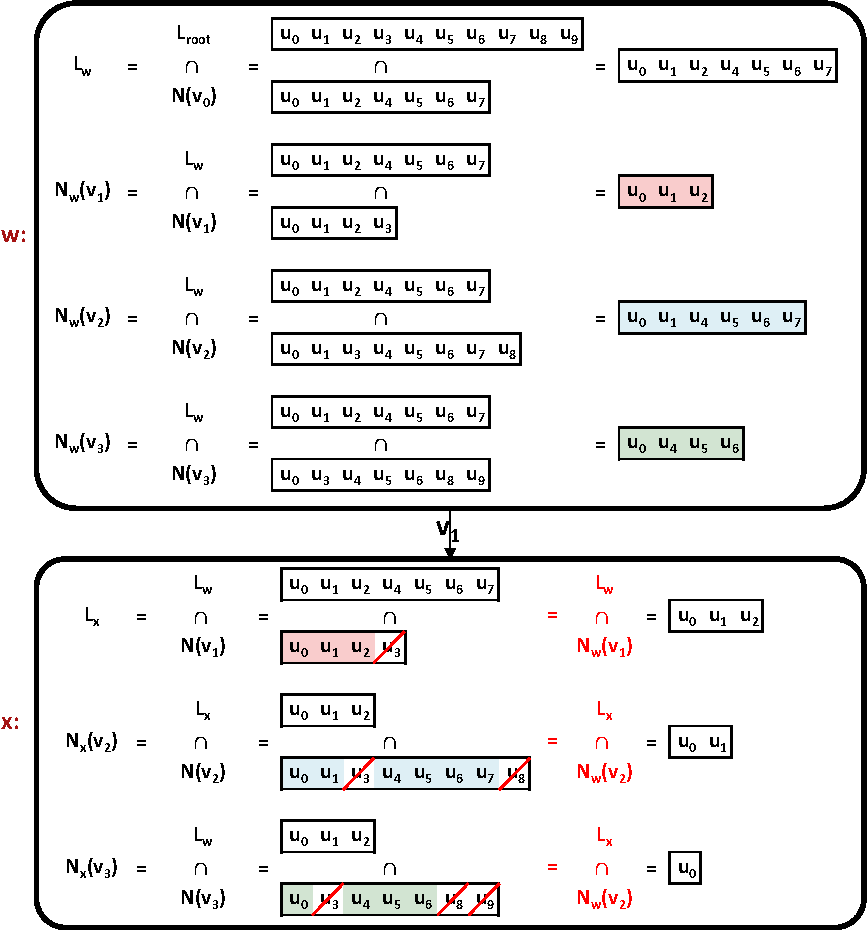
\includegraphics[width=0.85\linewidth]{adambe/eg_redundancy}
%   % \vspace{0.05in}
% 	\caption{完整邻居访问导致的冗余计算示例}

% 	\label{fig:ada_motivation_2}

% \end{figure}

% \begin{example}
%   图~\ref{fig:ada_motivation_2}展示了图~\ref{fig:ada_eg_tree}所示枚举树中父节点$w$和子节点$x$中涉及的部分集合交集运算。这些计算包括对每个节点的集合$L$以及对每个节点候选集合$C$的计算过程。

%   在每个节点的计算中,我们发现存在由无关顶点引起的冗余计算。除了我们提到的$L_x$的计算过程外,其他集合运算过程同样存在冗余。例如,在子节点$x$的集合$N_x(v_2)$的计算过程中,我们可以通过访问父节点中候选顶点$v_2$的局部邻居$N_w(v_2)$得到正确的计算结果,避免对$v_2$的全部邻居$N(v_2)$进行访问。因为根据推导$N_x(v_2) = L_x\cap N(v_2) = L_x \cap L_w \cap N(v_2) = L_x \cap N_w(v_2)$,我们知道$N(v_2)\setminus N_w(v_2)$中的顶点$u_3$和$u_8$不会对$N_x(v_2)$的计算结果产生影响,涉及冗余计算。同理,$N_x(v_3)$计算过程中的$u_3$,$u_8$和$u_9$也涉及冗余计算。
  
% \end{example}

\section{AdaMBE算法设计与实现}

为了克服现有方法的不足,本节提出了基于局部计算子图的优化方法和基于位图的动态子图方法,以提升极大二分团枚举算法的效率。其中,基于局部计算子图的优化方法利用计算子图中的局部邻居信息,加速了极大二分团枚举算法的核心操作,同时减少了算法中的无效的顶点访问、集合运算以及枚举节点;而基于位图的动态子图方法利用位图加速了小计算子图中的集合运算,在集合运算性能和访存效率之间进行了良好的折中。最终,我们结合这两种技术,形成了高效的自适应极大二分团枚举算法AdaMBE。

\subsection{基于局部计算子图的优化方法}
\label{subsec:ada_design_2}

为了减少原图中的无效顶点访问,我们提出了一种基于局部计算子图的优化方法,即LCG(Local Computational subGraph)方法。其核心设计思想是\textbf{动态缓存局部计算子图,并基于该子图重新设计算法的核心操作},以提升枚举性能。具体而言,我们观察到每个节点需要计算候选顶点的局部邻居作为中间结果。因此,我们可以通过缓存候选顶点的局部邻居这一中间结果,来得到局部计算子图。这里,顶点$v$在节点$x$中的\emph{局部邻居}被定义为$N(v)$和$L_x$的交集,\emph{在本章中被记作$N_x(v)$}。为了提升计算性能,我们利用计算子图中的局部邻居重新设计了~\ref{subsec:baseline}节算法~\ref{alg:se_mbe}中的三个核心操作:

(1) \textit{减少计算$R'$ 和 $C'$时的无效\emph{顶点}访问。} 
在当前的极大二分团枚举算法中,计算当前节点的集合$R'$ 和 $C'$通常涉及计算每个候选顶点 $v_c$ 在当前节点的局部邻居 $L' \cap N(v_c)$。这一过程对应于算法~\ref{alg:se_mbe} 中的第6和第8行。该过程默认访问顶点$v_c$ 在原图中的邻居$N(v_c)$。然而,根据第\ref{subsec:ada_limitation_vertex}节中的观察 O2,我们采用了一种优化策略:使用顶点 $v_c$ 在当前节点父节点 $x$ 对应计算子图中的局部邻居 $N_x(v_c)$ 替代原图中邻居$N(v_c)$的访问。由于计算子图中的局部邻居 $N_x(v_c)$ 通常规模较小,远远少于原图中的全部邻居 $N(v_c)$,因此计算 $L' \cap N_x(v_c)$ 的开销明显低于计算 $L' \cap N(v_c)$。为了便于获取顶点的局部邻居,我们将每次计算候选顶点$v_c$在当前节点局部邻居$L' \cap N(v_c)$这一中间结果缓存起来,以避免不必要的顶点访问。

局部邻居 $L' \cap N(v_c)$ 的计算是现有极大二分团枚举算法中的必要步骤。通过缓存局部邻居这一中间结果,我们可以得到每个节点对应的计算子图,进而消除计算子图之外的无效顶点访问,提高枚举效率。具体而言,通过缓存局部邻居,我们平均减少了97.1\%的计算子图外的无效顶点访问,如图~\ref{fig:ada_motivation_redundancy}所示。鉴于极大二分团枚举问题是计算密集型任务,内存使用较少,利用一些额外的内存来存储局部邻居以减少运行时间是值得的。

(2) \textit{消除计算$L'$时的重复\emph{集合}运算。}
我们注意到现有极大二分团枚举算法中存在重复的集合运算。具体而言,根据算法~\ref{alg:se_mbe},计算当前节点集合$L'$的过程$L \cap N(v')$(第4行)与其父节点$(L, R, C)$计算候选顶点$v'$局部邻居的过程(第8行)完全相同。因此,通过缓存$v'$的局部邻居,我们可以避免重复计算$L'$的集合运算。尽管这个问题在现有的极大二分团枚举算法中很常见,但还没有得到解决。

(3) \textit{节点生成前裁剪无效\emph{枚举节点}。}
根据我们的观察,我们注意到每个顶点的局部邻居始终对应于枚举节点的集合 $L$,如算法~\ref{alg:se_mbe} 的第4行所示。因此,我们可以知道相同的局部邻居将导致具有相同集合 $L$ 的节点,从而产生无效枚举节点。具体而言,当节点 $q$ 是节点 $p$ 的子节点且顶点 $v$ 的局部邻居大小在两个节点中相等,即 $|N_p(v)| = |N_q(v)|$ 时,节点 $p$ 可以安全地裁剪掉通过遍历顶点 $v$节点生成的无效枚举节点。 因为$N_p(v)$ 总是包含 $N_q(v)$ 中的所有顶点,邻居大小的相等即可表明 $N_p(v)$ 和 $N_q(v)$ 是相同的。因此,我们可以通过确保每个局部邻居仅生成一个节点来实现枚举节点的剪枝。





% 为了减少因访问顶点的完整邻居而产生的冗余,我们提出了一种基于局部计算子图的优化方法,即LCG(Local Neighbor Caching)方法。其核心设计思想是\textbf{动态缓存候选顶点的局部邻居,并重新利用这些中间结果},以避免对非活跃邻居进行大量内存访问。该方法有效地减少了三种类型的冗余:

% (1) \emph{\textit{粗粒度冗余。}}
% 这种冗余指的是对应非极大二分团的\textbf{节点},如图~\ref{fig:ada_eg_tree} 所示的节点$z$和节点$r$。最近的极大二分团枚举算法优化工作侧重于裁剪这些节点以减少此类冗余~\cite{iMBEA14,PMBE20,ooMBE22}。LCG 方法为这些努力提供了补充。

% (2) \emph{\textit{中等粒度冗余。}}
% 这种冗余源于枚举过程中重复的\textbf{集合}交集运算。从算法~\ref{alg:se_mbe} 中可以观察到,当父节点$p$遍历顶点$v_c$生成子节点$c$时,节点$p$中计算$v_c$局部邻居的过程始终与节点$c$中计算集合$L_c$的过程相同,即$L_p\cap N(v_c)$。例如,图~\ref{fig:ada_motivation_2}显示父节点 $w$使用$L_w\cap N(v_1)$计算$N_w(v_1)$,同时子节点$x$也使用$L_w\cap N(v_1)$计算$L_x$,这两个计算过程完全相同,存在冗余。尽管这种冗余在现有的极大二分团枚举算法中普遍存在,但没有算法试图解决这个问题。

% (3) \emph{\textit{细粒度冗余。}}
% 这种冗余是指非活跃\textbf{顶点}的内存访问,即不是候选顶点的局部邻居的顶点。~\ref{subsec:ada_limitation} 节详细介绍了这个问题。其中表~\ref{tbl:ada_motivation} 表显示超过 90\% 的内存访问涉及这些无用的顶点。然而,现有工作忽视了这个重要的限制。

% LCG方法通过缓存并利用候选顶点的局部邻居来实现。接下来,我们将通过解决三种冗余问题的方式进行详细阐述具体的实现细节:

% (1) 为了减少由非极大二分团对应节点带来的粗粒度冗余,我们利用局部邻居这一中间结果进行剪枝。具体而言,当同一候选顶点$v$的局部邻居在父节点$p$和子节点$c$中保持不变时,我们可以安全的裁剪掉由节点$p$遍历顶点$v$生成的节点。这是因为根据极大二分团枚举算法深度优先搜索的策略,父节点将会产生一个非极大二分团。关于这一点,我们将在~\ref{subsec:gmbe_prune}节中的定理~\ref{theorem:gmbe_prune}处进行详细描述。在这种情况下,我们将 $N_p(v)$和$N_c(v)$存储在相同的内存空间中,以减少内存使用,因为它们是相同的。

% (2)为了避免由重复集合交集运算引起的中等粒度冗余,我们将当前节点内每个候选顶点的局部邻居存储在它们各自对应的子节点中。当父节点$p$遍历候选顶点$v$生成子节点$c$时,子节点$c$可以直接访问$L_c$而无需进行冗余计算,因为$L_c$始终等同于预先存储的局部邻居 $N_c(v)$。

% (3)为了避免由于非活跃顶点的内存访问而导致的细粒度冗余,我们决定对所有局部邻居进行缓存。这样一来,我们可以只访问顶点的局部邻居,而不是整个邻居集合。具体而言,子节点$c$ 可以通过使用父节点$p$缓存的局部邻居来计算每个$C_c$ 中的顶点$v$ 的局部邻居。这一计算过程可以表达为$N_c(v) = L_c \cap N(v) = L_c \cap (L_p \cap N(v)) = L_c \cap N_p(v)$,其中$L_c$ 总是$L_p$的子集。这一设计可使我们更高效地利用已经计算过的中间结果,从而进一步减少内存访问和计算量。



\begin{figure} [H]
	\centering
  \vspace{0.1in}
	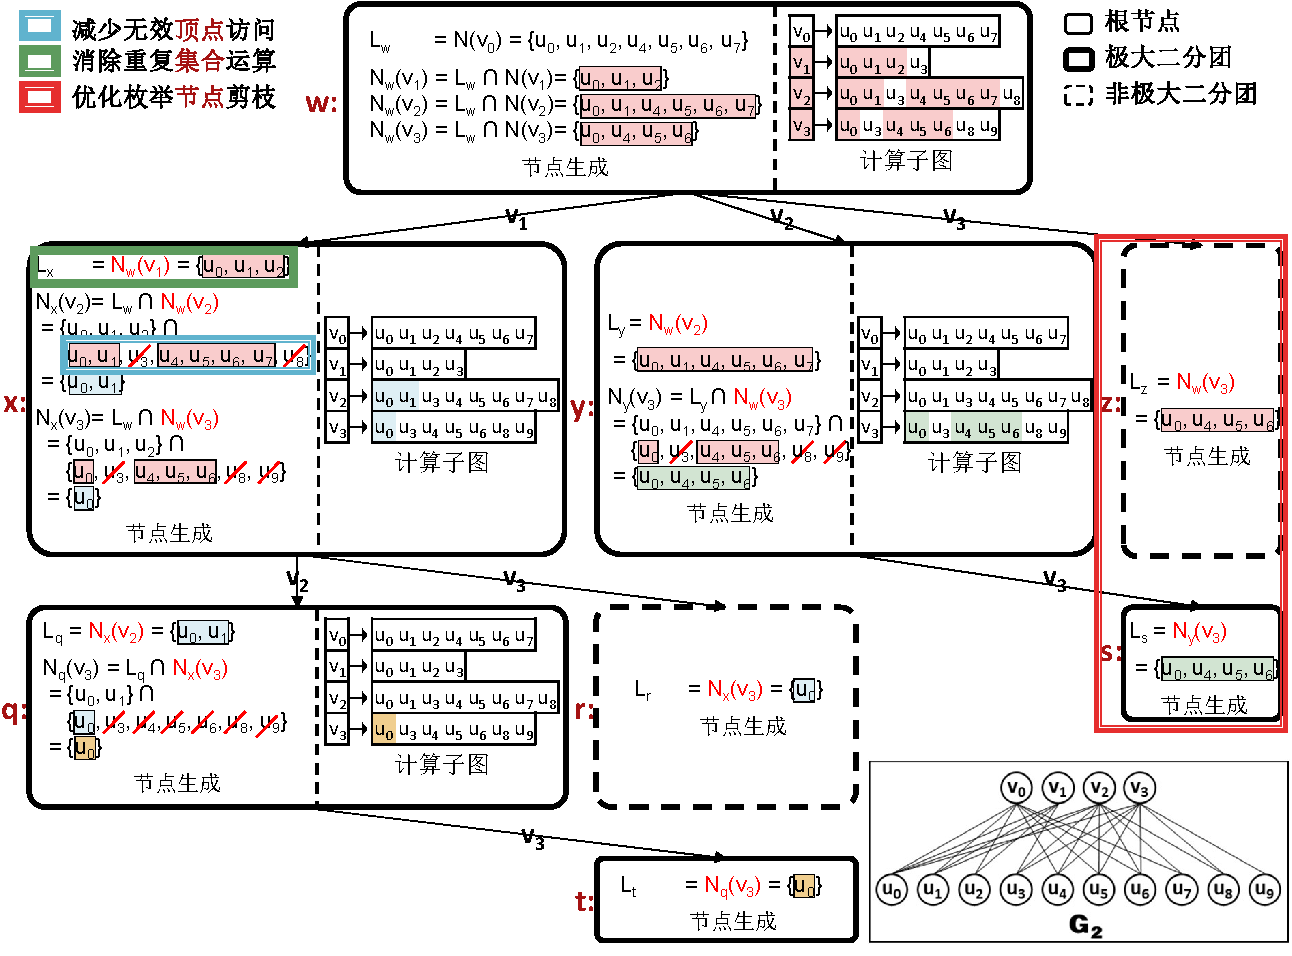
\includegraphics[width=\linewidth]{adambe/eg_design2_new}
  % \vspace{0.05in}
	\caption{基于局部计算子图的优化方法示例}

	\label{fig:ada_design2}
\end{figure}

接下来,我们用一个实例进行说明:

\begin{example}
	图~\ref{fig:ada_design2}展示了在图~\ref{fig:ada_eg_tree} 中节点 $w$ 为根节点的子树中使用 LCG 方法的过程。LCG方法在枚举过程中,将候选顶点的局部邻居默认缓存到当前节点对应的计算子图中。为了区分不同节点对应的计算子图和局部邻居,我们使用不同的颜色进行标示。

	首先,LCG方法通过访问顶点在计算子图中的局部邻居,避免了对顶点全部邻居的遍历,从而消除了在当前计算子图之外的无效顶点访问。例如,节点$x$利用其父节点$w$的计算子图中缓存的局部邻居$N_w(v_2)$计算$N_x(v_2)$,有效地避免了对当前计算子图之外的无效顶点的访问,如$u_3$和$u_8$。其次,LCG方法通过直接访问父节点的计算子图获取当前节点的集合$L$,避免了重复的集合交集运算。例如,节点$x$通过直接访问其父节点$w$的计算子图中$v_1$的局部邻居,即$N_w(v_1)$,得到$L_x$。最后,LCG方法通过比较父节点和子节点的中候选顶点的局部邻居大小来实现节点剪枝。例如,节点$w$通过比较节点$w$和$y$中顶点$v_3$的局部邻居大小相等,即$|N_w(v_3)| = |N_y(v_3)| = 4$,实现对由顶点$v_3$产生的节点$z$的剪枝。
	



  % 图~\ref{fig:ada_design2} 中展示了以图~\ref{fig:ada_eg_tree} 中节点 $w$ 为根节点的子树中使用 LCG 方法的过程。LCG方法在枚举过程中,将候选顶点的局部邻居动态缓存到该节点的子节点中。例如节点$w$将其候选顶点集$C_w$ 中全部顶点的局部邻居$N_w(v_1)$、$N_w(v_2)$和$N_w(v_3)$分别存放在节点$x$,$y$ 和 $z$ 中,通过对局部邻居的缓存,有效减少了来自无效枚举节点、重复集合运算以及无效顶点访问三个层面的冗余计算。
		
	% 对于非极大二分团对应节点导致的粗粒度冗余,我们采用了根据候选顶点邻居变化进行裁剪的策略。例如,节点 $w$ 对其子节点 $z$ 进行了裁剪,因为针对生成节点 $z$ 的候选顶点 $v_3$,其局部邻居大小在当前节点 $w$ 和子节点 $y$ 中保持不变,即 $|N_w(v_3)| = |N_y(v_3)| = 4$。	对于由重复集合交集运算引起的中等粒度冗余,我们根据LCG方法中局部邻居缓存的设计思路,已经将候选顶点的局部邻居存储在相应的子节点中,有效地避免了这种冗余。例如,节点 $w$ 在其子节点 $x$、$y$ 和 $z$ 中分别存储了局部邻居 $N_w(v_1)$、$N_w(v_2)$ 和 $N_w(v_3)$。这样每个节点就可以直接利用缓存的局部邻居来访问其集合 $L$,比如节点 $x$ 可以通过访问缓存的局部邻居 $N_w(v_1)$ 来获取 $L_x$。对于非活跃顶点访问所导致的细粒度冗余,我们通过仅访问缓存的候选顶点局部邻居而非完整邻居的方式来最小化这类冗余。例如,节点 $q$ 将使用局部邻居 $N_w(v_2)$ 来计算 $N_x(v_2)$,而不是完整邻居 $N(v_2)$。这一方法避免了访问与计算无关的顶点,如 $u_3$ 和 $u_8$。







	% 我们根据局部邻居大小进行裁剪,去除非极大二分团的节点(粗粒度冗余)。例如,节点 $w$ 将其子节点 $z$ 进行裁剪,因为节点 $w$ 知道当前遍历顶点 $v_3$ 的局部邻居大小保持不变,即 $|N_w(v_3)| = |N_y(v_3)| = 4$。我们通过在子节点中存储候选顶点的局部邻居来避免重复的集合交集操作(中等粒度冗余)。例如,节点 $w$ 在其子节点 $x$、$y$ 和 $z$ 中分别存储局部邻居 $N_w(v_1)$、$N_w(v_2)$ 和 $N_w(v_3)$。这样每个节点就可以直接使用缓存的局部邻居访问其集合$L$,比如节点 $x$ 可以将 $L_x$ 访问为 $N_w(v_1)=L_x$。我们通过仅利用缓存的局部邻居而非完整邻居来最小化内存访问(细粒度冗余)。例如,节点 $q$ 使用局部邻居 $N_w(v_2)$ 来计算 $N_x(v_2)$,而非完整邻居 $N(v_2)$。这一方法避免了访问不相关顶点,如 $u_3$ 和 $u_8$。
\end{example}

LCG方法的主要贡献包括以下两点:

\begin{enumerate}
	\item \textbf{提升中间结果的利用率。}
	在现有的极大二分团枚举算法中,局部邻居作为必要的中间结果,扮演着至关重要的角色。LCG方法通过缓存这些中间结果来动态缓存节点的计算子图,并利用该子图实现了对枚举过程的优化。虽然LCG方法需要额外的内存来存储局部邻居,但是如图~\ref{fig:ada_motivation_redundancy}所示,这一方法平均减少了无效顶点的内存访问量达到了97.1\%,从而提升了效率。鉴于内存并非计算密集型极大二分团枚举问题的瓶颈,使用额外的内存空间来缩短计算时间是值得的。
	


	\item \textbf{同时解决枚举过程中的多种问题。}
	在缓存了计算子图之后,我们充分利用了这些子图,解决了枚举过程中的多个问题,包括无效顶点访问、重复集合运算和无效枚举节点。与传统的优化方法只注重剪枝无效枚举节点不同,LCG方法通过巧妙地利用缓存的计算子图,成功地解决了极大二分团枚举中的无效顶点访问问题和重复集合运算问题。当前,图挖掘领域的最新算法开始关注重复集合运算导致的计算低效性问题~\cite{Graphpi20,GPMredundancy23}。然而,与这些现有方法相比,我们提出的LCG方法额外关注了更细粒度的顶点访问层面的问题,并成功解决了这些问题,为解决图挖掘领域中无效顶点访问的问题提供了全新的思路。

\end{enumerate}



\subsection{基于位图的动态子图方法}
\label{subsec:ada_design_1}

为了优化邻接表上高昂的集合运算开销,我们提出了一种基于位图的动态子图方法,即BDS(Bitmap-based Dynamic Subgraph)方法。其核心思想是\emph{利用位图加速小计算子图} \emph{中的集合运算操作}。如~\ref{subsec:ada_representation}节所述,计算子图的存储结构是计算效率和内存效率之间的权衡。因此,BDS方法采用混合图存储结构:对于原图或者大的计算子图,我们用邻接表来表示,以提高内存效率;对于小的计算子图,我们用动态建立的位图来表示,以提高集合运算效率。

具体而言,我们观察到枚举过程中计算子图是不断缩小的。根据算法~\ref{alg:se_mbe}所述,新节点$(L',R',C')$中的集合$L'$和$C'$中的全部顶点均源自父节点$(L, R, C)$对应的集合$L$和$C$(第4、8-9行),即$L'\subset L$且$C'\subset C$。由此可知,随着枚举过程的深入,根据节点内集合$L$和$C$产生的计算子图也在不断缩小。因此,我们设计的BDS方法可以在当前节点对应的计算图大小小于给定的阈值时动态建立子位图,并充分发挥位图在高效集合交集运算方面的优势,在以当前节点为根节点的子枚举树中重用该子位图。



% 为了优化邻接表上高昂的集合交集运算开销,我们提出了一种基于位图的动态子图方法,即BDS(Bitmap-based dynamic subgraph)方法。不同于传统方法只采用单一的图存储方式,BDS方法\textbf{融合了邻接表和位图两种图存储结构},利用邻接表表示整个二分图,在枚举过程中使用位图创建小规模子图。通过这种方式,我们可以借助高效的位运算加速在极大二分团枚举过程中的集合交集运算。

% BDS方法的设计基于我们的核心观察:\emph{在枚举过程中,由活跃顶点诱导的计算图总} \emph{是在不断缩小}。具体而言,在枚举过程中,根据算法~\ref{alg:se_mbe},新节点$(L',R',C')$中的集合$L'$和$C'$中的全部顶点均是源自父节点$(L, R, C)$对应的集合$L$和$C$(第4、8-9行),即$L'\subset L$且$C'\subset C$。由此可知,随着枚举过程的深入,节点内集合$L$和$C$中活跃顶点诱导的计算图也在不断缩小。因此,我们设计的BDS方法可以在当前节点对应的计算图大小小于我们给定的阈值时动态建立子位图,并充分发挥位图在高效集合交集运算方面的优势,在以当前节点为根节点的子枚举树中重用该子位图。

BDS方法的实现细节,我们通过回答以下两个关键问题的方式进行详细阐述:

\textit{(1)如何创建和利用基于位图的计算子图?}对于给定的节点$(L^*, R^*, C^*)$,我们利用位图从原始图$G(U, V, E)$中创建计算子图$CG_{bit}(U',V',E')$。为了构建$U'$,我们选择了所有$L^*$中的顶点。这是因为$U \setminus L^*$中的顶点无法存在于$L'$中,不会对算法~\ref{alg:se_mbe}(第4、6、8行)中的中间结果产生影响。为了构建$V'$,我们选择了不包括$R^*$内顶点在内的所有与$L^*$中任意顶点相连的顶点,存储为$\bigcup_{u \in L^*}N(u) - R^*$。这是因为未与$L^*$中任何顶点相连的顶点不能存在于$C'$ 或 $\Gamma(L')$中,也不能对算法~\ref{alg:se_mbe}中的中间结果产生影响。我们从$V'$中排除$R^*$中的顶点,因为它们总是出现在所有子节点的$R'$和$\Gamma(L')$中(第12行),这样可以减少不必要的计算。$E'$包含原图内$U'$ 和$V'$之间的所有边。当 $U'$的大小(即$|L^*|$)小于某个给定的小的\emph{常数$\tau$}时,算法中的每个集合操作都可以通过按位与操作(\&)在$O(\tau) = O(1)$ 的时间内完成。我们通过检查对于所有$V'$中的顶点$v$是否满足$L' \cap N(v) = L'$来计算$\Gamma(L')$。这一节点检查过程需要$O(\tau \Delta(U))=O(\Delta(U))$ 的时间,因为$V'$最多包含$\tau \Delta(U)$ 个顶点,且每个顶点的集合交集运算只需 $O(1)$ 的时间。综上所述,创建和利用基于位图的计算子图使得能够加速极大二分团枚举算法中的集合运算过程,其中每个节点的计算时间为$O(\Delta(U))$。

\textit{(2)何时创建基于位图的计算子图? }为了优化集合交集操作并提高计算效率,在考虑当前节点 $(L^*, R^*, C^*)$的情况下,我们在满足以下条件时创建基于位图的计算子图:当$|L^*|$小于或等于阈值$\tau$且$C^*$ 不为空时。这些条件至关重要,因为$|L^*|$直接影响集合交集所需的时间,而$C^*$ 影响位图在子节点中的重用次数。然而,选择适当的阈值$\tau$是具有挑战性的。较大的$\tau$会增加集合交集的时间(即$O(\tau)$)和每个子图的内存使用。相反,较小的$\tau$会导致创建更多小的子图,从而限制了在子节点中位图的重用机会。因此,在确定$\tau$时,我们必须在集合交集计算的效率和位图的利用之间取得平衡。根据我们在~\ref{subsec:ada_eval_sensitivity}节的实验,我们建议将阈值$\tau$设为64,因为这种情况下每次操作只需要对两个64位长长整数(long long integer)进行高效的按位与操作。



\begin{figure} [H]
	\centering
  \vspace{0.1in}
	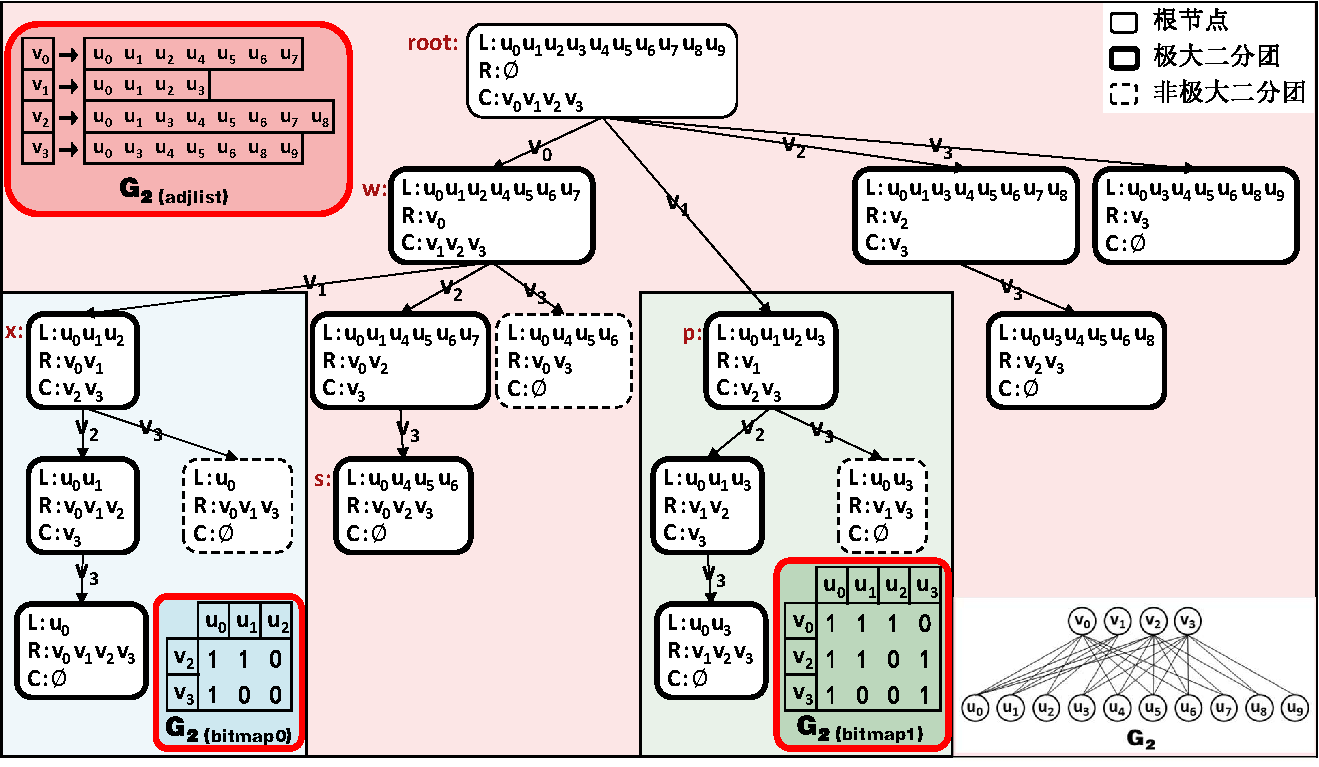
\includegraphics[width=0.98\linewidth]{adambe/eg_design_1}
  % \vspace{0.1in}
	\caption{基于位图的动态子图方法示例}

	\label{fig:ada_design1}
\end{figure}


% 接下来,我们用一个实例进行说明:

\begin{example}
  % 图~\ref{fig:ada_design1}中展示了在二分图$G_2$上应用BDS方法进行极大二分团枚举的过程。在这个例子中,阈值$\tau$设置为4。最初,图$G_2$使用邻接表作为默认方法存储(标记为$G_{2 (adjlist)}$)。当我们从节点$w$进入节点$x$时,我们观察到$|L_x| = 3 < \tau < |L_w| = 7$ 且 $C_x$不为空集,因此,我们在节点$x$处创建了基于位图的计算子图$CG_{2 (bit0)}$。在$CG_{2 (bit0)}(U_0, V_0, E_0)$中,$U_0$包含$L_x$中的所有顶点,即$u_0$、$u_1$和$u_2$。$V_0$包含$v_2$和 $v_3$,因为它们与$L_x$中的某些顶点有连接。$V_0$不包含$v_0$和$v_1$,因为它们属于$R_x$。因此,节点$x$的所有子节点都可以通过利用$CG_{2 (bit0)}$中的位图加速集合交集运算。类似地,在节点$p$处,我们创建另一个基于位图的计算子图$CG_{2 (bit1)}$,该子图加速了$p$节点所有后继节点的计算过程。特别地,对于节点$s$,尽管$|L_s| = 4 = \tau$,但由于节点$s$的候选顶点集$C_s$为空,这意味着如果此位图被创建,将没有子节点可以重用此位图,因此我们不在节点$s$处创建子图。
	
	图~\ref{fig:ada_design1}展示了在二分图$G_2$上应用BDS方法进行极大二分团枚举的过程。在这个示例中,设定阈值$\tau$为4。初始时,图$G_2$采用邻接表作为默认存储方式(标记为$G_{2 (adjlist)}$)。当节点$w$遍历顶点$v_1$进入到节点$x$时,我们观察到$|L_x| = 3 < \tau < |L_w| = 7$,且$C_x$非空,因此在节点$x$处生成基于位图的计算子图$CG_{2 (bit0)}$。在$CG_{2 (bit0)}(U_0, V_0, E_0)$中,$U_0$包含$L_x$中的所有顶点,即$u_0$、$u_1$和$u_2$。$V_0$包含$v_2$和$v_3$,因为它们与$L_x$中的某些顶点相连,但不包括$v_0$和$v_1$,因为它们属于$R_x$。因此,利用$CG_{2 (bit0)}$中的位图,可以加速计算节点$x$的所有后继节点的集合交集运算。类似地,在节点$p$处,创建另一个基于位图的计算子图$CG_{2 (bit1)}$,以加速计算$p$节点所有后继节点的过程。特别地,在节点$s$处,尽管$|L_s| = 4 = \tau$,但由于节点$s$的候选顶点集$C_s$为空,意味着若创建子位图,将没有子节点能够重复利用,因此在节点$s$处不生成该子位图。
  
\end{example}

\begin{algorithm} [H]
  \begin{algorithmic}[1]
    \normalsize
    \REQUIRE 当前枚举节点$(L_p, R_p, C_p)$,基于位图的计算子图 $CG_{bit}$
    \ENSURE 所有以节点$(L_p, R_p, C_p)$为根节点的枚举子树中的极大二分团


    \renewcommand{\algorithmicwhile}{\textbf{procedure}}
    \renewcommand{\algorithmicdo}{\textbf{:}}
    
    \WHILE{\textsf{AdaMBE\_search\_bit}($L_p, R_p, C_p, CG_{bit}$)}
    \FOR{$v' \in C_p$}
      \STATE $L_q \leftarrow L_p$ \h{\&} $N_{bit}(v')$;
      \STATE $is\_maximal \leftarrow$ \textbf{True};
      \FOR{$v'' \in U_{bit} \setminus (R_p \cup C_p$)}
        \IF{$L_q = L_p$ \h{\&} $N_{bit}(v'')$}
          \STATE $is\_maximal \leftarrow$ \textbf{False} ;
        \ENDIF
      \ENDFOR
      \IF{$is\_maximal$}
        \STATE $R_q \leftarrow R_p;$ $C_q \leftarrow \emptyset$ ;
        \FOR{$v_c \in C_p$}
          \IF{$L_q$ \h{\&} $N_{bit}(v_c) = L_q$}
            \STATE $R_q \leftarrow R_q \cup \{v_c\}$ ;
          \ELSIF{$L_q$ \h{\&} $N_{bit}(v_c) \neq 0$}
            \STATE $C_q \leftarrow C_q \cup \{v_c\}$ ;
          \ENDIF
        \ENDFOR
        \STATE 输出极大二分团 $(L_q, R_q)$ ;
        \STATE \textsf{AdaMBE\_search\_bit}($L_q, R_q, C_q, CG_{bit}$) ;
      \ENDIF
      \STATE $C_p \leftarrow C_p \setminus \{v'\} $ ;
    \ENDFOR
    \ENDWHILE

  \end{algorithmic}
  \caption{基于位图的动态子图方法运行过程}
  \label{alg:adambe_bit}
\end{algorithm}




% 算法~\ref{alg:adambe_bit}中给出了基于位图的动态子图方法运行过程。该过程的输入包括当前枚举节点 $(L_p, R_p, C_p)$ 以及根据 BDS 方法实现细节(1)建立的基于位图的计算子图$CG_{bit}$。与算法~\ref{alg:se_mbe}类似,该算法依次遍历$C_p$中的每个顶点$v'$ 生成新的枚举节点(第2行)并递归地调用\textsf{biclique\_search\_adambe\_bit}过程(第20行)。利用基于位图的计算子图$CG_{bit}$,该过程通过按位与(\&)操作取代高开销的集合运算操作,高效地实现节点检查(第4-9行)和节点生成(第3、11-18行)过程。值得注意的是,在递归过程中,计算子图$CG_{bit}$被反复使用(第1、20行)。

算法~\ref{alg:adambe_bit}描述了基于位图的动态子图方法的运行过程。该过程的输入包括当前枚举节点 $(L_p, R_p, C_p)$,以及基于 BDS 方法实现细节(1)建立的基于位图的计算子图 $CG_{bit}$。类似于算法~\ref{alg:se_mbe},该算法按顺序遍历 $C_p$ 中的每个顶点 $v'$,生成新的枚举节点(第2行),并递归调用 \textsf{biclique\_search\_adambe\_bit} 过程(第20行)。通过利用基于位图的计算子图 $CG_{bit}$,该过程通过位运算操作(\&)代替高开销的集合运算操作,以高效实现节点检查(第4-9行)和节点生成(第3、11-18行)过程。我们用红色字体标记了位运算的使用。值得注意的是,在递归过程中,计算子图 $CG_{bit}$ 会被反复重用(第1、20行)。

  BDS方法的主要贡献包括以下两点:

  \begin{enumerate}
    \item \textbf{结合两种不同图存储结构的优势。} 在选择图的存储结构时,我们需要在计算效率和内存效率之间取得平衡。对于大规模二分图,我们采用邻接表存储结构,因为它具有较好的内存效率;而对于小规模子图,则使用位图存储结构,因为它具有较好的计算效率。我们的BDS方法在原始图和较大的子图上继续沿用邻接表存储,有效地控制了在极大二分团枚举过程中的内存使用。早期的极大二分团枚举算法研究在小规模图$G(U, V, E)$上使用了位图存储~\cite{lcmmbc07,iMBEA14}。然而,即使在这些小规模图中,如果$U$内的顶点数量不足够小,每次按位集合交集操作的时间复杂度仍为$O(|U|)$,而非$O(1)$。因此,在许多情况下,直接采用位图存储方式未必能达到理想的计算效率。相反,BDS方法通过设置一个小的阈值$\tau$限制$U$的大小,保证每次集合操作的完成时间为$O(1)$,从而保证了计算效率。
    
    \item \textbf{充分利用二分图的特点。} 相较于通用图,基于位图的计算子图技术在二分图中有着特殊的优势。具体而言,对于只有一个顶点集$V$的通用图$G(V,E)$,确定何时创建位图是一项挑战。具体地,如果通用图顶点数$|V|$很大且稀疏,创建位图会导致内存使用效率低下;相反,如果$|V|$很小,则位图无法得到充分重用。最近的子图枚举算法的研究~\cite{Graphset23}指出,由于子位图技术的使用往往会带来巨大的内存开销,因此基于位图的计算子图优化技术仅应用在少数几项工作中~\cite{Sandslash21,Kclique22,g2miner22}。幸运的是,在具有两个不相交顶点集$U$和$V$的二分图$G(U,V,E)$中,我们可以通过小的$|U|$实现高效的内存使用,并通过大的$|V|$实现位图的有效利用。因此,BDS方法通过充分利用二分图的独特特性,显著改进了极大二分团枚举问题。
  
\end{enumerate}


\subsection{AdaMBE算法}
\label{subsec:ada_design_all}

结合LCG方法和BDS方法,我们提出了一种自适应的极大二分团枚举算法,简称为AdaMBE(Adaptive Maximal Biclique Enumeration)。该算法的核心思想是根据极大二分团枚举的不同阶段,分别采用这两种方法:在原图和大计算子图中采用LCG方法,利用动态缓存的计算子图提高计算效率;而在小计算子图中采用BDS方法,通过位图加速其中的集合运算操作。LCG方法和BDS方法能够在不同规模计算子图的场景下实现优势互补。此外,针对一个二分图 $G(U,V,E)$,AdaMBE会根据顶点的邻居大小对集合 $V$ 中的所有顶点进行初始排序。我们将在~\ref{subsec:ada_eval_sensitivity} 节通过实验展示其高效性。








\begin{algorithm} [H]
  \begin{algorithmic}[1]
    \normalsize

    \REQUIRE 二分图 $G(U,V,E)$
    \ENSURE 所有极大二分团
    \STATE 将$V$中顶点按照邻居数量递增排序;
    \STATE \textsf{AdaMBE\_search}($U, \emptyset, V, G$) ;
     
    \renewcommand{\algorithmicwhile}{\textbf{procedure}}
    \renewcommand{\algorithmicdo}{\textbf{:}}
    

    \WHILE{\textsf{AdaMBE\_search}($L_p, R_p, C_p, CG_p$)}
      \IF{$|L_p|\le \tau$ 并且 $C_p$ 不为空}
        \STATE 创建基于位图的计算子图 $CG_{bit} (U_{bit}, V_{bit}, E_{bit})$ ;
        \STATE \textsf{AdaMBE\_search\_bit}($L_p, R_p, C_p, CG_{bit}$) ;
        \STATE \textbf{Return} ;
      \ENDIF
      \FOR{$v' \in C_p$}
        \STATE $L_q \leftarrow$ \hh{$N_p(v')$} ; $R_q\leftarrow R_p$ ; $C_q \leftarrow \emptyset$ ; $CG_q \leftarrow \emptyset$ ;
        \FOR{$v_c \in C_p$}
          \STATE \hh{$N_q(v_c)$} $\leftarrow L_q$ $\cap$ \hh{$N_p(v_c)$} ;
          \STATE $CG_q$\textsf{.insert}(\hh{$N_q(v_c)$}) ;
          \IF{\hh{$N_p(v_c)$} = \hh{$N_q(v_c)$}}
            \STATE $CG_q$\textsf{.delete}(\hh{$N_p(v_c)$}) ;
          \ENDIF
          \IF{\hh{$N_q(v_c)$} = $L_q$}
            \STATE $R_q \leftarrow R_q \cup \{v_c\}$ ;
          \ELSIF{\hh{$N_q(v_c)$} $\neq \emptyset$}
            \STATE $C_q \leftarrow C_q \cup \{v_c\}$ ;
          \ENDIF
        \ENDFOR
        \IF{$R_q = \Gamma(L_q)$}
          \STATE 输出极大二分团 $(L_q, R_q)$ ;
          \STATE \textsf{AdaMBE\_search}($L_q, R_q, C_q, CG_q$) ;
        \ENDIF
        \STATE \textsf{free}($CG_q$) ; $C_p \leftarrow C_p \setminus \{v'\} $;
      \ENDFOR
    \ENDWHILE 

  \end{algorithmic}
  \caption{AdaMBE算法}
  \label{alg:adambe}
\end{algorithm}






算法~\ref{alg:adambe}描述了AdaMBE算法的执行过程。对于二分图 $G(U,V,E)$,AdaMBE选择将$V$中顶点按照邻居数量递增排序(第1行)。随后,AdaMBE从根节点$(U,\emptyset,V)$开始,递归地调用\textsf{biclique\_search\_adambe}过程,初始时默认当前计算子图为原图 $G$ (第2行)。\textsf{biclique\_search\_adambe}过程的输入包括当前枚举节点 $(L_p, R_p, C_p)$以及节点$p$对应的计算子图$CG_p$(第3行)。对于$|L_p| > \tau$ 的较大的计算子图,AdaMBE利用局部邻居信息加速枚举过程(第9-28行)。这些局部邻居信息以蓝色字体标记。对于$|L_p| \le \tau$ 的较小的计算子图,AdaMBE动态创建子位图,并调用算法~\ref{alg:adambe_bit}中的\textsf{biclique\_search\_adambe\_bit}过程(第4-8行)。根据~\ref{subsec:ada_eval_sensitivity}节的实验结果,AdaMBE默认将阈值$\tau$设置为64。

% 算法~\ref{alg:ambea}详细描述了AMBEA。具体而言,对于二分图$G(U,V,E)$,在~\ref{subsec:order}节所示的顶点排序方法中,AMBEA选择将$V$中顶点按照邻居数量递增排序 (第1行),因为在这种顺序下AMBEA算法性能最优。我们将通过下一节的实验证明这一结论。随后,该算法从根节点$(U,\emptyset,V)$开始,按顺序遍历$V$中的顶点$v$,并递归地调用\textsf{biclique\_search\_ambea}过程 (第2-4行)。在枚举过程中,AMBEA同时利用了ASE树中的低成本节点检查技术和AMP方法中的主动顶点合并剪枝技术。通过两种技术的有机结合,AMBEA高效地减小了计算空间,并取得了良好的计算性能。


% 为了清晰表述,我们在算法~\ref{alg:adambe_bit}中给出了基于位图的动态子图方法运行过程,并在算法~\ref{alg:adambe}中给出完整的AdaMBE算法。


% 结合BDS方法和LCG方法,我们设计了一种自适应的极大二分团枚举算法,简称为AdaMBE(Adaptive Maximal Biclique Enumeration)。该算法的基本思想是在极大二分团枚举过程的不同阶段分别应用这两种方法,即使用BDS方法处理基于小图的子位图,使用LCG方法处理基于原图的邻接表。这是因为在小图场景下,BDS方法可以通过位运算提升集合交集运算的效率,在处理小图时性能优于LCG方法;而在大原始图的场景下,LCG方法有效填补了BDS方法没有优化的空白。此外,对于一个二分图$G(U,V,E)$,AdaMBE会根据它们的邻居大小对集合$V$中的所有顶点进行初始排序,我们将在~\ref{subsec:ada_eval_sensitivity} 节通过实验展示其高效性。

接下来,我们从时间复杂度和空间复杂度两个方面对AdaMBE进行讨论。

\textbf{时间复杂度:} 与第~\ref{ch:aggressive_mbe}章介绍的AMBEA算法相似,AdaMBE算法的时间复杂度由顶点排序时间和集合枚举树生成时间组成。其中,按照顶点度数升序排列的时间复杂度为$O(|V|log(|V|))$,在邻接表中每个节点的计算时间为$O(|E|)$,而在位图中每个节点的计算时间为$O(\Delta(U))$。为了量化算法的计算时间,我们用$\beta$表示枚举树中节点的数量,包括输出极大二分团的节点和产生非极大二分团的节点。我们将$\beta$分解为两部分,即$\beta_0$表示基于邻接表计算的枚举节点,而$\beta_1$表示基于子位图计算的枚举节点。最终,我们得到AdaMBE的计算复杂度为$O(|E|\beta_0 + \Delta(U)\beta_1 + |V|log(|V|))$。由于排序开销通常远小于生成集合枚举树的开销,因此,AdaMBE的时间复杂度可以简化为$O(|E|\beta_0 + \Delta(U)\beta_1 )$。在~\ref{subsec:ada_breakdown} 节的技术点分解评估实验中,我们观察到在真实数据集中,$\beta_1$通常占据了大部分的计算时间,因此相较于其他算法,AdaMBE表现出明显的性能提升。

\textbf{空间复杂度:} AdaMBE算法的空间复杂度可分为两部分:输入二分图所需空间和极大二分团枚举过程的空间。输入二分图所占用的空间为$O(|E|)$。在枚举过程中,LCG方法会动态保存顶点的局部邻居,构成原二分图的一个计算子图,因此每个节点所需空间为$O(|E|)$。由于枚举树的高度上限为$O(\Delta(V))$,因此AdaMBE的空间复杂度为$O(|E|+|E|\Delta(V)) = O(|E|\Delta(V))$,略高于当前最优算法的空间复杂度$O(|E|+|V|\Delta(V))$。这是因为AdaMBE算法中的LCG方法需要额外空间以增加局部邻居的重用性,从而提升计算性能。在~\ref{subsec:ada_overall} 节的整体评估实验中,我们观察到在测试的真实数据集上,AdaMBE的最大内存使用仅约为1GB,并且在大多数情况下,AdaMBE算法的内存占用仍低于先进算法PMBE和ooMBEA,因此相对于LCG方法带来的计算性能提升,其空间开销是可以接受的。

\textbf{并行扩展:} 为了进一步提升性能,我们在AdaMBE算法的基础上设计了其并行版本ParAdaMBE。受到并行算法ParMBE~\cite{parMBE19}的启发,ParAdaMBE利用Intel TBB库~\cite{tbb-code}的功能,为二分图集合$V$中的每个顶点$v$分配一个线程,负责处理由顶点$v$产生的子枚举树。这样,多个枚举树可以无重叠地并发计算。此外,只要存在额外线程可用,ParAdaMBE将对子枚举树对应的任务进行进一步分解。为了进一步提升并行计算资源的利用,ParAdaMBE通过循环展开技术有效并行化算法中的for循环,最大程度地利用并行性缩短算法的运行时间。

总而言之,与现有的极大二分团枚举方法忽视计算子图的特性不同,AdaMBE利用这些特性加速顶点访问和集合操作。它根据处理图的大小灵活选择LCG和BDS技术,优化了极大二分团枚举过程中最耗时的集合运算过程,显著改善了计算效率。

%尽管与GPU相比,\textit{\pname{}} 在CPU上的并行计算资源有限,但由于其高效的内存使用和自适应策略,在包含数十亿个极大二分团的数据集上仍然具有竞争力。


\section{实验评估}

\subsection{实验设置}

\textbf{实验环境设置:} 本节的全部实验均在一台配备有4个Intel Xeon(R) Gold 5318Y 2.10GHz CPU和128GB内存的服务器上完成,其中每个CPU拥有24个计算核心,共计96个计算核心。本次实验环境的操作系统为Linux kernel-5.4.0。在没有特殊说明的情况下,算法默认使用单个计算核心串行执行。鉴于现有算法在大规模数据集上很难在短时间内完成,我们将运行时间限制设置为48小时(INF)。

\textbf{比较算法:} 在我们的实验中,我们评估了串行和并行极大二分团枚举算法的性能。对于串行算法,我们将AdaMBE与过去五年中的三种最先进的算法进行了比较:FMBE~\cite{parMBE19},PMBE~\cite{PMBE20} 和 ooMBEA~\cite{ooMBE22}。对于并行算法,我们将 ParAdaMBE 与目前最先进的多线程并行算法ParMBE~\cite{parMBE19}进行比较。默认情况下,我们在同一台拥有 96 个核心的 CPU 的服务器上使用 96 个线程来运行ParAdaMBE和ParMBE。此外,为了深入评估本章提到的技术点,我们实现了一些算法变体,并在对应实验中详细描述。

\begin{table} [t]
	\centering    
	\setlength{\abovecaptionskip}{0cm}  
  \setlength{\belowcaptionskip}{-0.2cm}
	\caption{AdaMBE增加的实验数据集统计信息}      
	\label{tbl:ada_datasets}
	\setlength{\tabcolsep}{1pt}
	\begin{center}
				\normalsize{
		\begin{tabular}{|c|c|c|c|c|c|c|}
			\hline 
			\textbf{数据集} &\textbf{目录} &\textbf{类型} & \textbf{$|U(G)|$} & \textbf{$|V(G)|$} & \textbf{$|E(G)|$} &\textbf{极大二分团}\\
			\hline
			% Unicode (UL) & 特征关系 & 国家-使用-语言 &  614 & 254 & 1,255 & 460\\
			% UCforum (UF) & 交互关系 & 用户-发布-论坛 & 899 & 522 & 7,089 & 16,261\\
			% % Wikinews & 作者关系  & 用户-编辑-文章 & 41,747  & 1,572 & 109,218 & 44,444\\
			% %Writers (WR) & 作者关系 & 作者-出版-作品 & 89,355 & 46,213 & 144,340 & 57,222\\ 
			% MovieLens (Mti) & 特征关系 & 标签-属于-电影 & 16,528 & 7,601 & 71,154 & 140,266\\ 
			% Teams (TM) & 归属关系 & 队员-属于-团队 & 901,130 & 34,461 & 1,366,466 & 517,943 \\
			% ActorMovies (AM) & 归属关系 & 电影-出演-演员 & 383,640 & 127,823 & 1,470,404 & 1,075,444\\ 
			% Wikipedia (WC) & 特征关系 & 文章-属于-目录 &1,853,493 & 182,947 & 3,795,796 & 1,677,522 \\
      % YouTube (YG) & 归属关系 & 用户-属于-群组 & 94,238 & 30,087 & 293,360 & 1,826,587\\  
			% StackOverflow (SO) & 评分关系 & 作者-收藏-帖子 & 545,195 & 96,680 & 1,301,942 & 3,320,824 \\
			% DBLP (Pa) & 作者关系 & 作者-出版-作品 & 5,624,219 & 1,953,085 & 12,282,059 & 4,899,032\\
			% IMDB (IM) & 归属关系 & 电影-出演-演员 & 896,302 & 303,617 & 3,782,463 & 5,160,061\\
			% BookCrossing (BX) & 交互关系 & 用户-打分-书籍  & 340,523 & 105,278 & 1,149,739 & 54,458,953 \\
			% Github (GH) & 作者关系 & 用户-参与-工程 & 120,867 & 56,519 & 440,237 & 55,346,398 \\ 
      CebWiki (ceb) & 作者关系 & 用户-编辑-文章 & 8,483,068 & 3,132 & 11,792,890 & 263,138,916\\
			TVTropes (DBT) & 特征关系 & 作品-拥有-特征 & 87,678 & 64,415 & 3,232,134 & 19,636,996,096 \\ 
      \hline
      LJ10 & 归属关系 & 用户-属于-群组& 2,301,031& 1,421,088& 11,227,130& 7,430,705\\
			LJ20 & 归属关系 & 用户-属于-群组& 2,704,651& 2,357,485& 22,456,757& 61,836,924\\
			LJ30 & 归属关系 & 用户-属于-群组& 3,163,966& 2,889,804& 33,686,334& 343,257,225\\
			LJ40 & 归属关系 & 用户-属于-群组& 3,894,262& 2,992,774& 44,917,368& 1,524,229,722\\
			LJ50 & 归属关系 & 用户-属于-群组& 4,572,628& 3,057,410& 56,150,150& 6,387,845,280\\
      
      % \hline
			% LJ5 & 归属关系 & 用户-属于-群组& 1,837,928 & 853,994 & 5,610,437 & 2,181,295 \\
			% LJ10 & 归属关系 & 用户-属于-群组& 2,301,031 & 1,421,088 & 11,227,130 & 7,430,705 \\
			% LJ15 & 归属关系 & 用户-属于-群组& 2,548,619 & 1,912,139 & 16,843,216 & 22,727,251 \\
			% LJ20 & 归属关系 & 用户-属于-群组& 2,704,651 & 2,357,485 & 22,456,757 & 61,836,924 \\
			% LJ25 & 归属关系 & 用户-属于-群组& 2,812,080 & 2,771,510 & 28,068,423 & 151,468,807 \\

			% LiveJournal & 归属关系 & 用户-属于-群组 & 7,489,073 & 3,201,203 & 112,307,385 & -\\
			% WebTrackers & Hyperlink & Domain-Inclusion-Tracker & 27,665,730 & 12,756,244 & 140,613,762 & -\\ 
			\hline
		\end{tabular}
				}
	\end{center}
	\vspace{-0.1in}
\end{table}



\textbf{数据集:} 为了准确评估本章提出的技术,我们同时使用了真实数据集和合成数据集。为了进一步探索 AdaMBE 在包含超过 1 亿极大二分团的大数据集上的性能,我们在上一章实验中的表~\ref{tbl:datasets} 的基础上额外增加了大数据集,如表~\ref{tbl:ada_datasets} 所示。其中,真实数据集 CebWiki 和 TVTropes 来源于 KONECT 仓库~\cite{konect},TVTropes数据集包含的极大二分团数量超过了196亿。合成数据集是在大数据集 LiveJournal ($|U|$=7,489,073, $|V|$=3,201,203, $|E|$=112,307,385) 上分别采样 10\%、20\%、30\%、40\% 和 50\% 的边所生成,分别记作 LJ10、LJ20、LJ30、LJ40 和 LJ50,其中 LJ30、LJ40 和 LJ50 中的极大二分团数量均超过 1 亿。大数据集 LiveJournal 也来自于 KONECT 仓库。

\subsection{整体评估}
\label{subsec:ada_overall}

\textbf{常规数据集上的性能评估:} 为了验证我们提出的算法的整体效率,我们在12个常规数据集上测量了所有竞争对手的运行时间和内存使用情况。运行时间不包括从磁盘加载图的时间,内存使用表示相应进程的最大内存占用。


% \begin{figure} [H]
% 	\vspace{0.05in}
%   \centering
%   \subfloat[AdaMBE在常规数据集上的整体运行时间评估 (对数形式)]{
% 		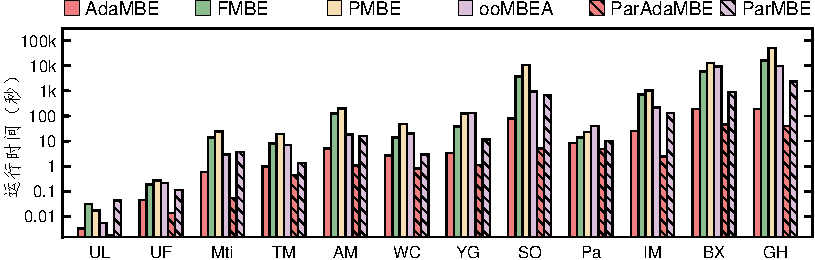
\includegraphics[width=0.95\linewidth]{adambe/overall_time}
% 		\label{fig:ada_overall_time}
% 	}
% 	\vspace{0.05in}
% 	\\
%   \subfloat[AdaMBE在常规数据集上的整体内存使用评估(对数形式)]{
% 		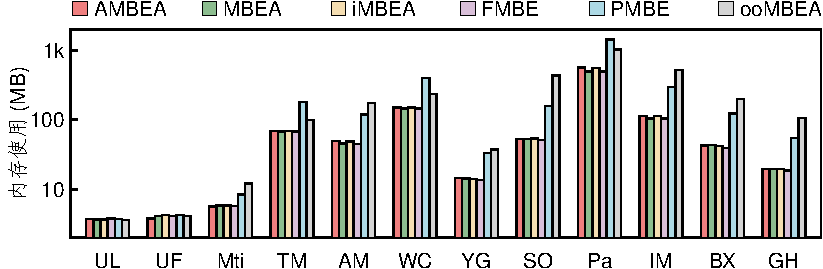
\includegraphics[width=0.95\linewidth]{adambe/overall_memory}
% 		\label{fig:ada_overall_memory}
% 	}
%   \caption{AdaMBE在常规数据集上的整体评估}
%   \label{fig:ada_overall}

% \end{figure}


\begin{figure} [H]
	\centering
  \vspace{0.05in}
	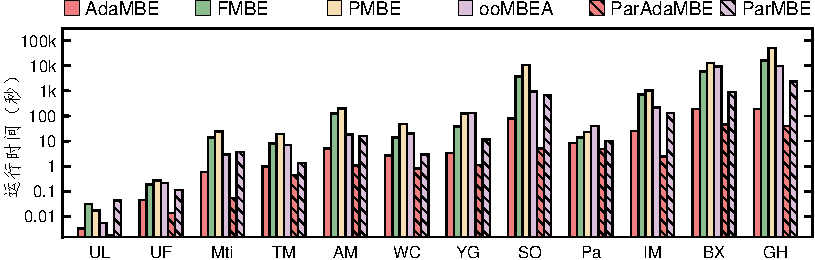
\includegraphics[width=\linewidth]{adambe/overall_time}
	\caption{AdaMBE在常规数据集上的整体运行时间评估 (对数形式)}

	\label{fig:ada_overall_time}
\end{figure}




图~\ref{fig:ada_overall_time}展示了在常规数据集上,AdaMBE、ParAdaMBE以及主流极大二分团枚举算法的运行时间对比。实验结果显示,在不同的数据集下,我们的串行算法 AdaMBE 在性能上始终比最接近的串行竞争对手快 1.6 到 49.7 倍,而并行算法 ParAdaMBE 则比 ParMBE 算法快 2.5 到 137.8 倍。特别值得注意的是,在耗时最长的数据集 Github 上,AdaMBE 仅用时 194 秒完成任务,而FMBE、PMBE 和 ooMBEA 算法分别需要 16,616 秒、51,647 秒和 9,639 秒。同样,ParAdaMBE 在 40 秒内完成任务,而 ParMBE 则需要超过 2,412 秒。这清楚地表明,与现有方法相比,AdaMBE 算法和ParAdaMBE算法在处理耗时较长的数据集时具有明显的性能优势,为大规模数据集上的极大二分团枚举任务提供了强大的技术支持。

\begin{figure} [t]
	\centering
   \vspace{0.05in}
	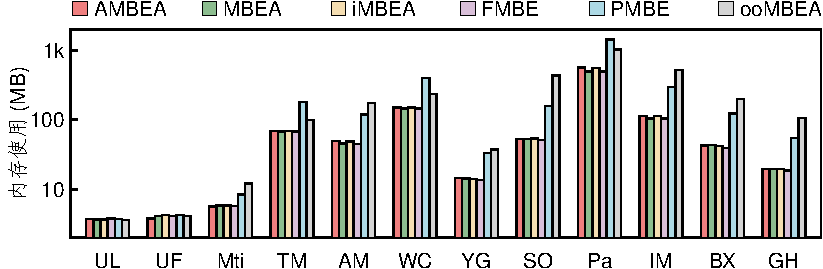
\includegraphics[width=\linewidth]{adambe/overall_memory}
	\caption{AdaMBE在常规数据集上的整体内存使用评估 (对数形式)}

	\label{fig:ada_overall_memory}
\end{figure}

图~\ref{fig:ada_overall_time}展示了在常规数据集上,AdaMBE、ParAdaMBE以及主流极大二分团枚举算法的内存使用对比。实验结果显示,与同类别中的其他算法相比,我们串行和并行算法的内存使用情况类似。同样以数据集Github为例,AdaMBE、FMBE、PMBE、ooMBEA、ParAdaMBE以及ParMBE的内存使用分别为32MB ,18MB,55MB,105MB,271MB 和	431MB。实验结果表明,虽然我们的AdaMBE在枚举过程中需要额外的内存来存储局部邻居,但它的内存使用仍然优于最近的串行算法 PMBE 和 ooMBEA。事实上,PMBE 和 ooMBEA 分别需要比 AdaMBE平均多1.4倍和1.9倍的内存,因为它们需要额外的内存来存储 CDAG 索引结构~\cite{PMBE20} 和多个静态子图~\cite{ooMBE22}。除此之外,尽管FMBE算法的内存使用量低于AdaMBE,但其运行时间却远远落后于AdaMBE。

\begin{figure} [H]
  \centering
	\vspace{0.05in}
	% \vspace{0.1in}
  \subfloat[CebWiki数据集上的运行时间评估
		% Evaluation on CebWiki. We report running time of all competitors excluding GMBE, which runs out of memory (OOM).
		]{
		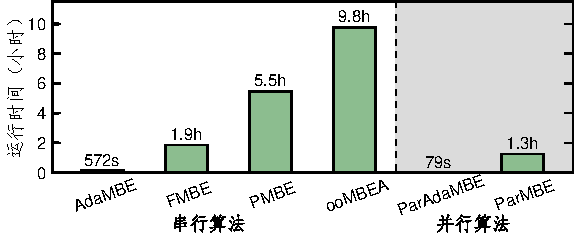
\includegraphics[width=0.8\linewidth]{adambe/cebwiki}
		\label{fig:ada_overall_cebwiki}
	}
	\\
  \subfloat[TVTropes数据集上48小时内算法输出的极大二分团数量
		% Evaluation on TVTropes. As only AdaMBE and \parpname{} complete within 48 hours, we report the maximal biclique count of competitors at 48 hours.
		]{
		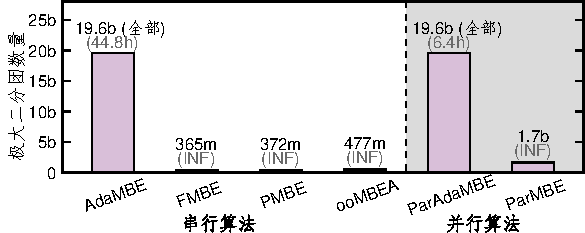
\includegraphics[width=0.8\linewidth]{adambe/tvtropes}
		\label{fig:ada_overall_tvtropes}
	}

  \caption{AdaMBE在超大数据集上的整体评估}
  \label{fig:ada_overall_large}
\end{figure}

\textbf{大规模数据集的评估:} 为了验证我们提出的算法在大规模二分图中的性能,我们在两个包含超过2亿个极大二分团的大规模数据集上测量了不同算法的运行时间。对于那些运行时间超过时间限制(48小时)的算法,我们报告它们在截止48小时时所产生的极大二分团数量。



图~\ref{fig:ada_overall_cebwiki} 展示了不同算法在 CebWiki 数据集上的运行情况。实验结果显示,AdaMBE 和 ParAdaMBE 的完成时间均小于10分钟,而其他现有算法的完成时间均超过1小时,最新的极大二分团枚举算法 ooMBEA 的运行时间甚至接近10小时。图~\ref{fig:ada_overall_tvtropes} 展示了不同算法在 TVTropes 数据集上的运行情况。实验结果显示,只有 AdaMBE 和 ParAdaMBE 在48小时内完成了对全部196亿极大二分团的枚举任务,完成时间分别为44.8小时和6.4小时。而其他比较算法在48小时内所枚举的极大二分团数量均不超过总数量的8.5\%。这清楚地表明,由于性能限制,现有方法难以在大规模数据集上得到有效应用。相比之下,AdaMBE 算法通过优化数据结构,充分利用计算子图动态变化的特性,在大规模二分图场景中表现出更为明显的优势。

\subsection{技术点分解评估}
\label{subsec:ada_breakdown}

为验证本章提出的具体优化技术,我们设计了消融实验,沿用整体评估中的运行时间和内存使用指标。具体而言,我们在8个极大二分团数量较多的常规数据集上,对
~\ref{subsec:ada_design_2}提到的LCG方法和
~\ref{subsec:ada_design_1}节提到的BDS方法
进行了分解评估。为了评估LCG和BDS方法的有效性,我们设计了三个变体:基准算法(禁用LCG和BDS)、AdaMBE-LCG(启用LCG的基准算法)和AdaMBE-BDS(启用BDS的基准算法)。我们比较了AdaMBE和这三个变体的运行时间和内存使用情况。随后,我们进行了单独的实验来深入分析LCG和BDS的性能提升原理。

% \begin{figure} [H]
%   \centering
% 	\vspace{0.05in}
%   \subfloat[运行时间评估(对数形式)]{
% 		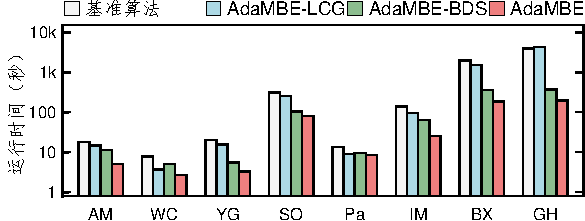
\includegraphics[width=0.8\linewidth]{adambe/breakdown_time}
% 		\label{fig:ada_breakdown_time}
% 	}
% 	\\
%   \subfloat[内存使用评估]{
% 		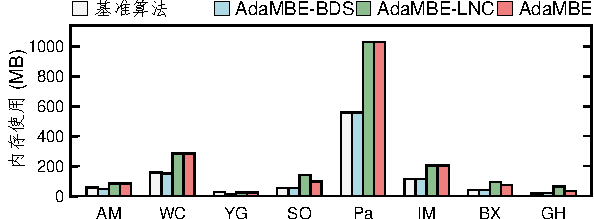
\includegraphics[width=0.8\linewidth]{adambe/breakdown_memory}
% 		\label{fig:ada_breakdown_memory}
% 	}

%   \caption{BDS、LCG方法的运行时间的内存使用分解评估}
%   \label{fig:ada_breakdown}
% \end{figure}



\begin{figure} [H]
	\centering
  % \vspace{0.05in}
	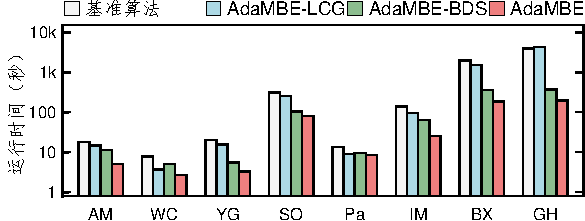
\includegraphics[width=0.8\linewidth]{adambe/breakdown_time}
	\caption{BDS、LCG方法的运行时间分解评估(对数形式)}

	\label{fig:ada_breakdown_time}
\end{figure}

\begin{figure} [H]
	\centering
  % \vspace{0.05in}
	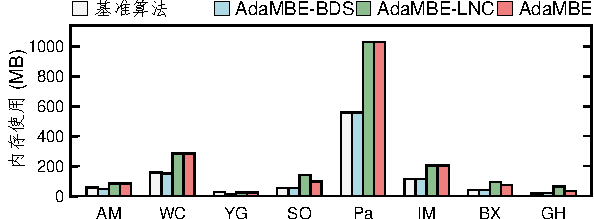
\includegraphics[width=0.8\linewidth]{adambe/breakdown_memory}
	% \vspace{-0.1in}
	\caption{BDS、LCG方法的内存使用分解评估(对数形式)}

	\label{fig:ada_breakdown_memory}
\end{figure}


\textbf{运行时间和内存使用评估:} 我们在包含更多极大二分团计数的8个常规数据集上评估了运行时间和内存使用情况。图~\ref{fig:ada_breakdown_time} 展示了BDS和LCG方法在运行时间上的分解评估。实验结果显示,AdaMBE中的LCG和BDS方法均对基准算法起到了加速效果。在8个测试数据集上,AdaMBE-LCG相比基准算法平均节约了24\%的执行时间,表明LCG方法也具有一定的加速效果。AdaMBE充分结合了这两种优化方法的优势,在所有测试数据集中性能都优于基准算法和其他变体。以Github数据集为例,AdaMBE 将基准算法的运行时间从 3,911 秒缩短至 194 秒。在StackOverflow、BookCrossing和Github等数据集上,相比基准算法,AdaMBE-BDS分别加速了3.0倍、5.6倍和10.7倍,显示出BDS方法在处理大数据集时的显著加速效果。图~\ref{fig:ada_breakdown_memory}展示了LCG和BDS方法在内存使用上的分解评估。实验结果显示,使用LCG方法的AdaMBE-LCG和AdaMBE算法的内存使用明显高于不使用LCG方法的基准算法和AdaMBE-BDS,这表明LCG方法在运行过程中增加了内存使用,与~\ref{subsec:ada_design_all}节中关于空间开销的讨论结果一致。然而,考虑到极大二分团枚举问题是一个计算密集型问题,内存需求相对较低,因此增加一定的内存使用来加速计算过程是一个明智的策略。具体来说,在Github数据集上,AdaMBE-BDS和AdaMBE的运行时间分别为367秒和194秒,这表明LCG方法很好地补充了BDS方法。总体而言,在所有测试数据集上,AdaMBE 的内存使用都未超过1.3 GB(在 CebWiki 数据集上),额外的内存使用是可以接受的。



\begin{figure} [t]
	\centering
  % \vspace{0.05in}
	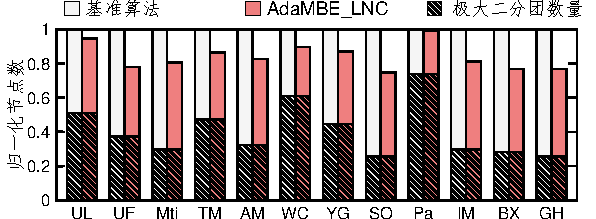
\includegraphics[width=0.8\linewidth]{adambe/breakdown_design2}
  %  \vspace{-0.1in}
	\caption{LCG方法的节点剪枝效率}

	\label{fig:ada_breakdown_design2}
\end{figure}

% \textbf{LCG方法的效果:}  为了更深入评估~\ref{subsec:ada_design_2}节中LCG方法,我们分别评估了该方法利用局部计算子图信息增强三个关键操作的有效性。首先,LCG方法消除了计算子图之外的所有顶点访问,并因此较少了大多数数据集上超过90\%的顶点访问,如~\ref{subsec:ada_limitation_vertex}节的图~\ref{fig:ada_motivation_redundancy}所示。其次,LCG方法由于LCG方法利用缓存的邻居信息,彻底避免了关于候选顶点局部邻居和节点集合$L$的重复集合交集计算,详见~\ref{subsec:ada_design_2}节。最后,LCG方法在图~\ref{fig:breakdown_design2} 中展现了节点剪枝的效率:它平均减少了12个常规数据集中对应非极大二分团的25\%的节点。与现有极大二分团仅关注枚举节点剪枝不同,LCG方法同时关注并减少了无效的顶点访问、集合运算和枚举节点。

\textbf{LCG方法的效果:} 为了更深入评估~\ref{subsec:ada_design_2}节中的LCG方法,我们分别评估了该方法利用局部计算子图信息重新设计算法的核心操作的有效性。首先,LCG方法消除了计算子图之外的所有顶点访问,并因此较少了大多数数据集上超过90\%的顶点访问,如~\ref{subsec:ada_limitation_vertex} 节的图~\ref{fig:ada_motivation_redundancy}所示。其次,LCG方法由于利用缓存的邻居信息,彻底避免了关于候选顶点局部邻居和节点集合$L$的重复集合交集计算,详见~\ref{subsec:ada_design_2} 节。最后,LCG方法在图~\ref{fig:ada_breakdown_design2} 中展现了节点剪枝的效率:该方法将12个常规数据集中对应非极大二分团的无效节点平均减少了25\%。
% 平均减少了12个常规数据集中25\%的对应非极大二分团的无效节点。
与现有极大二分团仅关注枚举节点剪枝不同,LCG方法同时关注并减少了无效的顶点访问、集合运算和枚举节点。

% 我们进行了实验验证其对~\ref{subsec:ada_design_2}节中提到的三种冗余的实际减少效果。首先,我们对基准算法和AdaMBE-LCG进行了节点枚举统计,将枚举节点根据是否形成极大二分团分为两部分,具体见图~\ref{fig:ada_breakdown_design2}。由于不同算法对同一数据集产生的极大二分团数量始终相同,图中使用阴影部分标识了重叠的对应极大二分团的部分。实验结果表明,LCG方法平均剪枝了25\%包含非极大二分团的节点,即减少了25\%的粗粒度冗余。其次,由于LCG方法利用缓存的邻居信息,彻底避免了关于候选顶点局部邻居和节点集合$L$的重复计算,完全消除了由重复集合操作引起的中等粒度冗余。最后,关于顶点访问级别的细粒度冗余,在~\ref{subsec:ada_limitation_vertex}节的图~\ref{fig:ada_motivation_redundancy}中显示,LCG方法在大多数数据集中减少了超过90\%的无关顶点访问,即减少了90\%的细粒度冗余。与现有的极大二分团枚举方法仅关注非极大二分团的粗粒度冗余不同,LCG方法通过同时处理所有三种冗余类型,有效提升了计算性能。






\begin{figure} [t]
	\centering
  % \vspace{0.05in}
	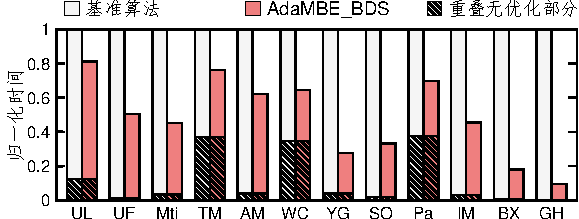
\includegraphics[width=0.8\linewidth]{adambe/breakdown_design1}
  % \vspace{0.05in}
	% \vspace{-0.1in}
	\caption{BDS方法下的运行时间分解}

	\label{fig:ada_breakdown_design1}
\end{figure}


% \textbf{BDS方法效果:} 为了评估BDS方法的加速效果,我们对基准算法和AdaMBE-BDS进行了运行时间分解分析,根据阈值$\tau$将每个算法的时间分解为两个部分,详见图~\ref{fig:ada_breakdown_design1}。具体而言,由于BDS方法仅优化$|L|$等于或小于阈值$\tau$的小节点$(L, R, C)$,图中标记了BDS方法无法优化的运行时间部分,包括重叠的算法初始化时间和大节点的计算时间。实验结果显示,BDS方法可以优化的小节点运行时间部分通常超过基准算法总时间的60\%,在BookCrossing和Github等大数据集上的占比超过了99\%;同时,在BDS方法可以优化的部分中,大多数数据集中小节点的运算时间缩短了50\%以上,特别是在Github数据集上,BDS方法实现了显著地缩短了91\%的小节点运算时间,使得AdaMBE-BDS相对于基准算法加速了10.7倍。

\textbf{BDS方法效果:} 为了评估BDS方法的加速效果,我们对基准算法和AdaMBE-BDS进行了运行时间分解分析。我们根据阈值$\tau$将每个算法的时间分解为两个部分,详见图~\ref{fig:ada_breakdown_design1}。具体而言,BDS方法仅优化了$|L|$等于或小于阈值$\tau$的小节点$(L, R, C)$,图中标记了BDS方法无法优化的运行时间部分,包括重叠的大节点的计算时间和算法初始化时间。实验结果显示,BDS方法可以优化的小节点运行时间部分通常超过了基准算法总时间的60\%,在BookCrossing和Github等大数据集上的占比更是超过了99\%。同时,在BDS方法可以优化的部分中,大多数数据集中小节点的运算时间缩短了50\%以上,特别是在Github数据集上,BDS方法实现了显著地缩短了91\%的小节点运算时间,使得AdaMBE-BDS相对于基准算法加速了10.7倍。

% \textbf{LCG方法的效果:} 为了评估LCG方法的影响,我们探讨了在~\ref{subsec:ada_design_2}节提到的三种冗余的减少效果。关于节点级别的粗粒度冗余,图~\ref{fig:ada_breakdown_design2}显示LCG方法平均减少了25\%的包含非极大二分团的节点。在集合操作级别的中等粒度冗余方面,LCG利用局部邻居缓存避免了重新计算集合$L$,从而完全消除了这种冗余。至于顶点级别的细粒度冗余,~\ref{subsec:ada_limitation}节的表~\ref{tbl:ada_motivation}显示,LCG方法在大多数数据集中减少了超过90\%的无关顶点访问。与之前只处理粗粒度冗余(即非极大二分团)的方法不同,LCG方法通过处理所有三种类型的冗余,提高了性能。

\subsection{敏感性测试}
\label{subsec:ada_eval_sensitivity}

我们对BDS方法中的阈值$\tau$选择、顶点的顺序选择以及算法的可扩展性进行了敏感性测试。

\begin{figure} [H]
	\centering
  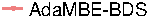
\includegraphics[width=0.2\linewidth]{adambe/sensitivity_threshold_legend} \\
	
  \subfloat[IMDB.]{
		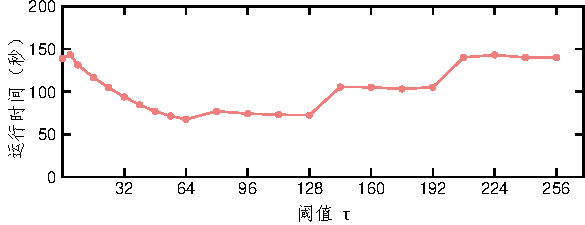
\includegraphics[width=0.7\linewidth]{adambe/sensitivity_threshold_im}
		\label{fig:sensitivity_threshold_im}
	}
	\\
	\subfloat[BookCrossing.]{
		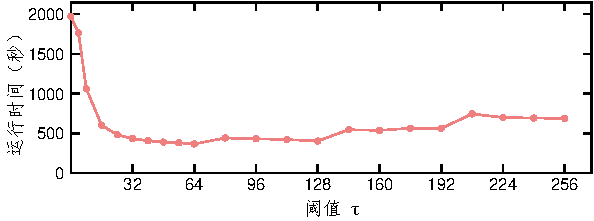
\includegraphics[width=0.7\linewidth]{adambe/sensitivity_threshold_bx}
		\label{fig:sensitivity_threshold_bx}
	}
	\\
  \subfloat[Github.]{
		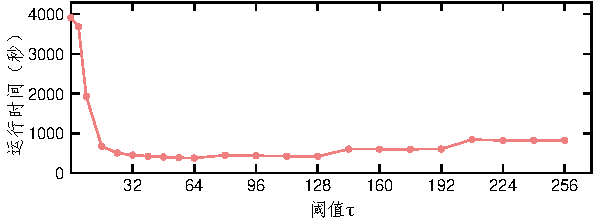
\includegraphics[width=0.7\linewidth]{adambe/sensitivity_threshold_gh}
		\label{fig:sensitivity_threshold_gh}
	}

	\caption{不同阈值$\tau$下BDS方法性能评估}
	\label{fig:ada_sensitivity_threshold}

\end{figure}



\textbf{BDS方法中阈值$\tau$的影响:} 为了确定~\ref{subsec:ada_design_1}节中的阈值$\tau$,我们在AdaMBE-BDS上进行了对不同$\tau$值(从4到256)的实验,该实验仅使用BDS方法。图~\ref{fig:ada_sensitivity_threshold} 展示了来自3个较大的常规数据集(即IMDB、BookCrossing和Github)的实验结果。随着$\tau$从4增加到64,运行时间持续减少。以BookCrossing数据集为例,当$\tau$为4时,算法运行时间为1,763秒;而当$\tau$为64时,算法运行时间仅为366秒。这是因为较大的$\tau$导致创建的子图减少,并且位图的重用增加。需要注意的是,在$\tau$不大于64时,每次集合交集运算只需对两个64位长整数进行一次按位与(\&)操作,因此集合交集运算时间保持不变。然而,当$\tau$超过64时,由于每次集合交集运算所需的时间增加,运行时间变得更长。此外,我们观察到当$\tau$是64的倍数时,运行时间较短,因为这些情况增强了位图的重用,并且每次集合交集运算所需时间相同。因此,AdaMBE将$\tau$的默认值设定为64。




\begin{figure} [H]
	\centering
	
  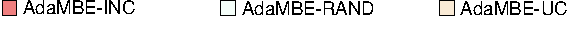
\includegraphics[width=0.8\linewidth]{adambe/order_legend}
  

  % \subfigure[Medium datasets.]{
		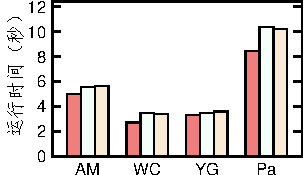
\includegraphics[width=0.42\linewidth]{adambe/order_medium}
	% }
  \quad
  % \subfigure[Large datasets.]{
		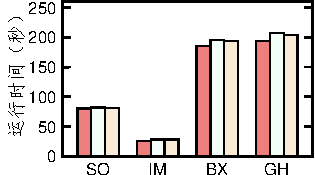
\includegraphics[width=0.42\linewidth]{adambe/order_large}
	% }

	\vspace{-0.1in}
	\caption{顶点顺序的性能评估}
	\label{fig:ada_order}

\end{figure}

\textbf{顶点排序的影响:} 为了确定AdaMBE算法的顶点初始排序方法,我们提出了三种变体:AdaMBE-INC、AdaMBE-RAND和AdaMBE-UC。这三种变体均以AdaMBE算法为基础,它们的区别在于集合$V$中顶点的初始排序方式不同。具体而言,AdaMBE-INC是根据邻居数量递增对顶点进行排序,AdaMBE-RAND则以随机顺序对顶点排序,而AdaMBE-UC采用了ooMBEA最新提出的单边顺序。在图~\ref{fig:ada_order} 中可以看到,在8个较大的常规数据集上,AdaMBE-INC始终优于AdaMBE-RAND和AdaMBE-UC,特别是在包含大量顶点的数据集上表现更为显著。举例来说,在DBLP数据集上,AdaMBE-INC、AdaMBE-RAND和AdaMBE-UC的运行时间分别为8.4秒、10.4秒和10.2秒。由此可见,按照顶点邻居数量递增排序的方法对性能提升具有积极作用,因此,AdaMBE默认采用基于邻居数量递增的顶点排序方式。

\begin{figure} [t]
	\centering
		\vspace{0.1in}
		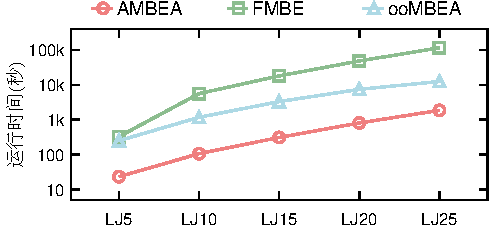
\includegraphics[width=0.7\linewidth]{adambe/scalability}
	\caption{可扩展性评估(对数形式)}
	\label{fig:ada_scalability}
\end{figure}



\textbf{可扩展性评估:} 为了评估AdaMBE算法的可扩展性,我们利用从LiveJournal数据集中生成的合成数据集进行了实验,该数据集包含超过1亿条边。在本实验中,我们分别对LiveJournal数据集进行了10\%、20\%、30\%、40\%和50\%的边抽样,并将它们分别命名为LJ10、LJ20、LJ30、LJ40和LJ50。表~\ref{tbl:ada_datasets} 中总结了这些数据集的统计信息。如图~\ref{fig:ada_scalability}所示,实验结果显示,随着数据规模的增加,不同算法的运行时间呈指数增长。在这些大型合成数据集上,AdaMBE的运行速度比所有串行竞争对手快11.4倍以上。具体而言,AdaMBE仅需6.6小时就能完成LJ50数据集中包含超过60亿个极大二分团的枚举任务,而其他竞争对手则需要48小时才能完成。由此可知,AdaMBE是处理大规模数据集的最佳选择。

\begin{figure} [H]
	\centering

	\subfloat[CebWiki]{
		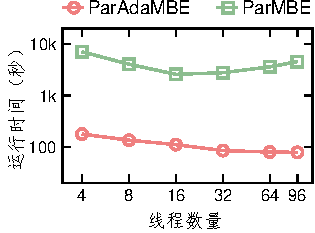
\includegraphics[width=0.47\linewidth]{adambe/parallel_ceb}
	}
  \quad
  \subfloat[Github]{
		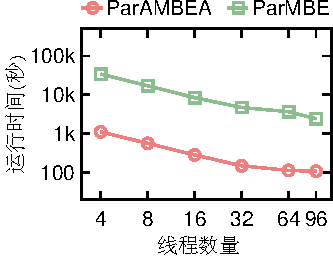
\includegraphics[width=0.47\linewidth]{adambe/parallel_gh}
	}

	\caption{并行性评估(对数形式)}
	\label{fig:ada_parallel}

\end{figure}

\textbf{并行性评估:} 为了评估AdaMBE算法的并行性能,我们比较了并行版本ParAdaMBE和当前最优的并行算法ParMBE在相同线程数量下的执行效率。考虑到ParMBE在TVTropes数据集上的极大二分团枚举任务无法在48小时内完成,我们在其余数据集中选择了运行时间最长的两个数据集:CebWiki和Github进行实验。我们分别使用4、8、16、32、64、96个线程在不同数据集上运行ParAdaMBE和ParMBE算法。考虑到实验服务器总共有96个计算核心,我们将线程数量上限设置为96。如图~\ref{fig:ada_parallel}所示,相较于ParMBE,ParAdaMBE表现出明显的性能优势。此外,随着线程数量的增加,ParAdaMBE的运行时间呈现线性下降的趋势,表明在各种线程配置下都能展现良好的性能。

% \textbf{并行性评估:}为了探索AMBEA的并行性,我们将其并行版本ParAMBEA与最先进的并行算法ParMBE进行比较。我们在四个运行时间最长的数据集上进行了实验:StackOverflow、IMDB、BookCrossing和Github。我们分别使用4、8、16、32、64、96个线程在不同数据集上分别运行ParAMBEA和ParMBE算法。由于实验服务器中共包含96个计算核,我们将线程数量上限设置为 96。如图~\ref{fig:ambea_paral}所示,ParAMBEA 相较于 ParMBE 具有明显的性能优势,运行时间缩短了 17.4-293.8 倍。同时,从图表中我们可以观察到,随着线程数量的增加,ParAMBEA 的运行时间几乎呈线性下降趋势,这意味着它可以有效地利用更多的计算资源来加速算法的执行。值得注意的是,通过并行化,我们成功将 BookCrossing 数据集上 AMBEA 算法的运行时间从 1,610 秒大幅缩短至仅需 51 秒。这个结果充分证明了ParAMBEA 在并行性能方面的优越性,并显示出其在大规模数据集上的应用潜力。



\section{本章小结}

本章提出了局部计算子图的优化方法(LCG)和基于位图的动态子图(BDS)方法,并结合这两种方法形成高效的极大二分团枚举算法AdaMBE,旨在解决极大二分团枚举问题中计算不规则、静态数据结构低效的挑战。首先,针对现有方法有算法使用静态图结构完成枚举,忽略枚举过程中子图动态变化的特性的问题,LCG方法通过动态缓存枚举过程中的计算子图的方式优化算法的枚举过程,减少无效的顶点访问、集合运算和枚举节点。其次,针对邻接表上集合运算的高开销问题,BDS方法在计算过程中动态生成子位图,以加速集合运算。通过利用位运算在子位图中进行集合运算,提升了效率。最后,将这两种技术整合,实现了AdaMBE算法及其并行版本ParAdaMBE。实验结果充分证明了AdaMBE算法的高性能,以及本章中所有优化方法的具体作用。